\documentclass[10pt,pdf,aspectratio=169,hyperref={unicode}]{beamer}

\usepackage[T2A]{fontenc}
\usepackage[utf8]{inputenc}
\usepackage[english,russian]{babel}
\usepackage{amssymb,amsfonts,amsmath}
\usepackage{graphicx}

\let\Tiny=\tiny

\setbeamertemplate{caption}[numbered]
\setbeamertemplate{theorems}[numbered]
\setbeamertemplate{navigation symbols}{}
\setbeamerfont{caption}{size=\footnotesize}

\definecolor{links}{HTML}{2A1B81}
\hypersetup{colorlinks,linkcolor=,urlcolor=links}

\usetheme{Pittsburgh}
\usecolortheme{whale}

\let\Definition\relax
\newtheorem{Definition}{Определение}
\let\Theorem\relax
\newtheorem{Theorem}{Теорема}

\newcommand{\inp}[1]{\input{../../out/#1}}
\newcommand{\characteristic}[2]{\inp{#1/characteristics/#2}}
\newcommand{\descriptive}[2]{\inp{#1/descriptive/#2}}
\newcommand{\test}[3]{\inp{#1/test/#2/#3}}
\newcommand{\normaldistr}{$\mathcal{N}(\descriptive{original}{mean}, \descriptive{original}{variance})$}
\newcommand{\resnormaldistr}{$\mathcal{N}(\descriptive{residual}{mean}, \descriptive{residual}{variance})$}

\logo{
\includegraphics[width=1cm,height=1cm,keepaspectratio]{Logo_BSU.jpg}}

\title{Анализ и прогнозирование гидрологических данных}
\subtitle[]{}
\author[Павлов Александр \hspace{0.2\textwidth} \insertframenumber\,/\,\inserttotalframenumber]{ Павлов Александр Сергеевич \\ \vspace{2em} \small{Научный руководитель: Цеховая Татьяна Вячеславовна \\Рецензент: Рафеенко Екатерина Дмитриевна} }

\institute[]{Кафедра Теории Вероятностей и Математической Статистики \vspace{2pt} \\ Факультет Прикладной Математики и Информатики \vspace{2pt} \\ Белорусский Государственный Университет }
\date{Минск, 2015}

\begin{document}

\begin{frame}[plain]
  \titlepage
\end{frame}

\section[Содержание]{}
\begin{frame}
  \frametitle{Содержание}
  \tableofcontents
\end{frame}

\section{Обзор реализованного программного обеспечения}

\begin{frame}
  \frametitle{Особенности}
  \begin{itemize}
    \item Доступно с любого устройства, имеющего доступ в интернет, по адресу \href{https://apaulau.shinyapps.io/batorino}{apaulau.shinyapps.io/batorino}
    \item Реализовано на языке программирования \textbf{R}
    \item Логически разделёно на три модуля
    \item Имеет простой, быстро расширяемый гибкий интерфейс
    \item Широкие графические возможности
    \item Проверка тестов и критериев
    \item Мгновенный отклик на изменение параметров
    \item Быстрая проверка различных моделей
  \end{itemize}
\end{frame}

\subsection{Модуль предварительного анализа}

\begin{frame}
  % \frametitle{Первичный анализ и описательные статистики}
  \frametitle{Модуль предварительного анализа}
    \begin{figure}[h]
    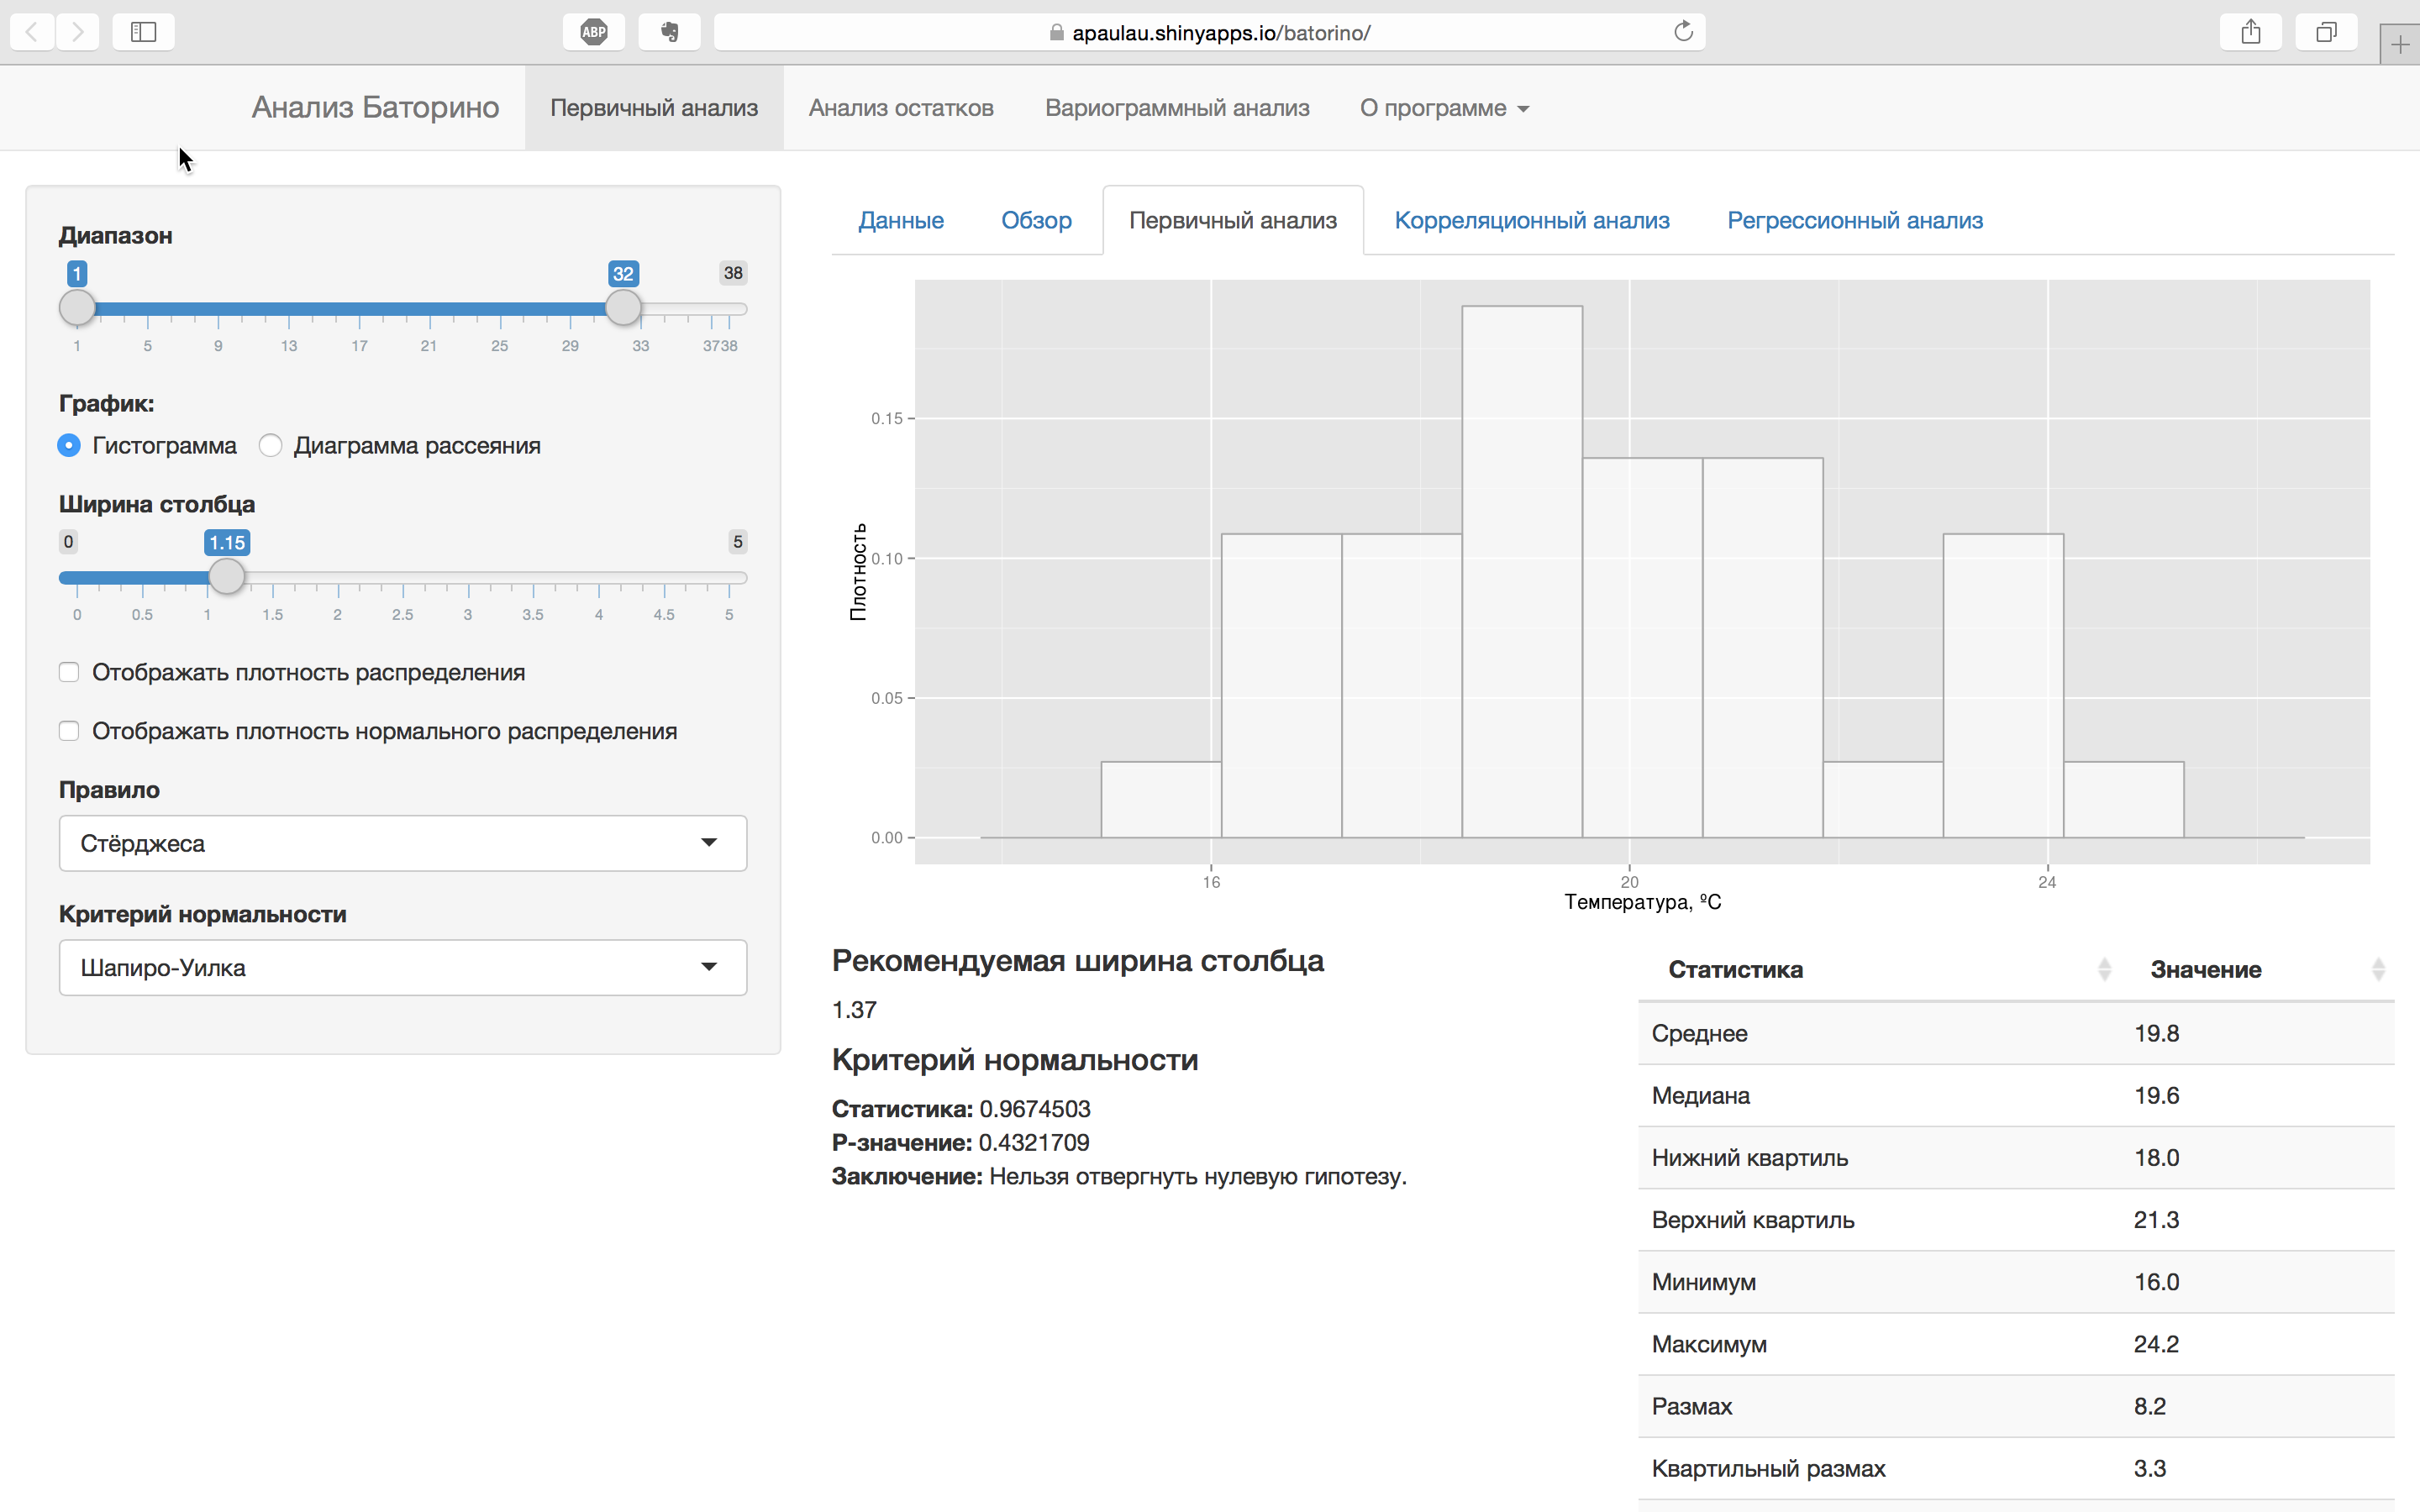
\includegraphics[width=0.75\textwidth]{../../figures/static/1_basis.png}
    \caption{Первичный анализ и описательные статистики}
  \end{figure}
\end{frame}

\begin{frame}
  % \frametitle{Корреляционный анализ}
  \frametitle{Модуль предварительного анализа}
  \begin{figure}[h]
    \center{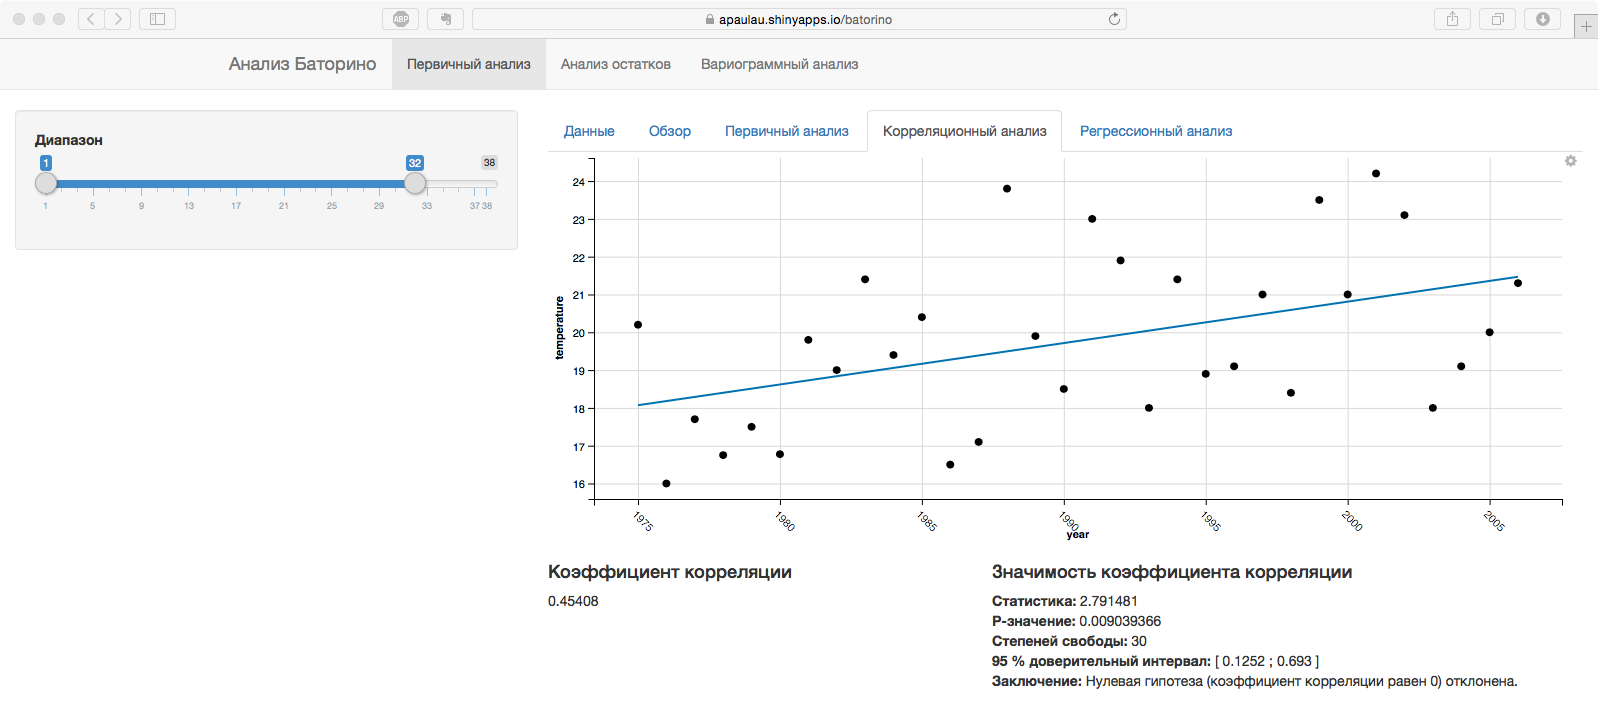
\includegraphics[width=0.75\textwidth]{../../figures/static/p_corr.png}}
    \caption{Корреляционный анализ}
  \end{figure}
\end{frame}

\begin{frame}
  % \frametitle{Регрессионный анализ}
  \frametitle{Модуль предварительного анализа}
    \begin{figure}[h]
    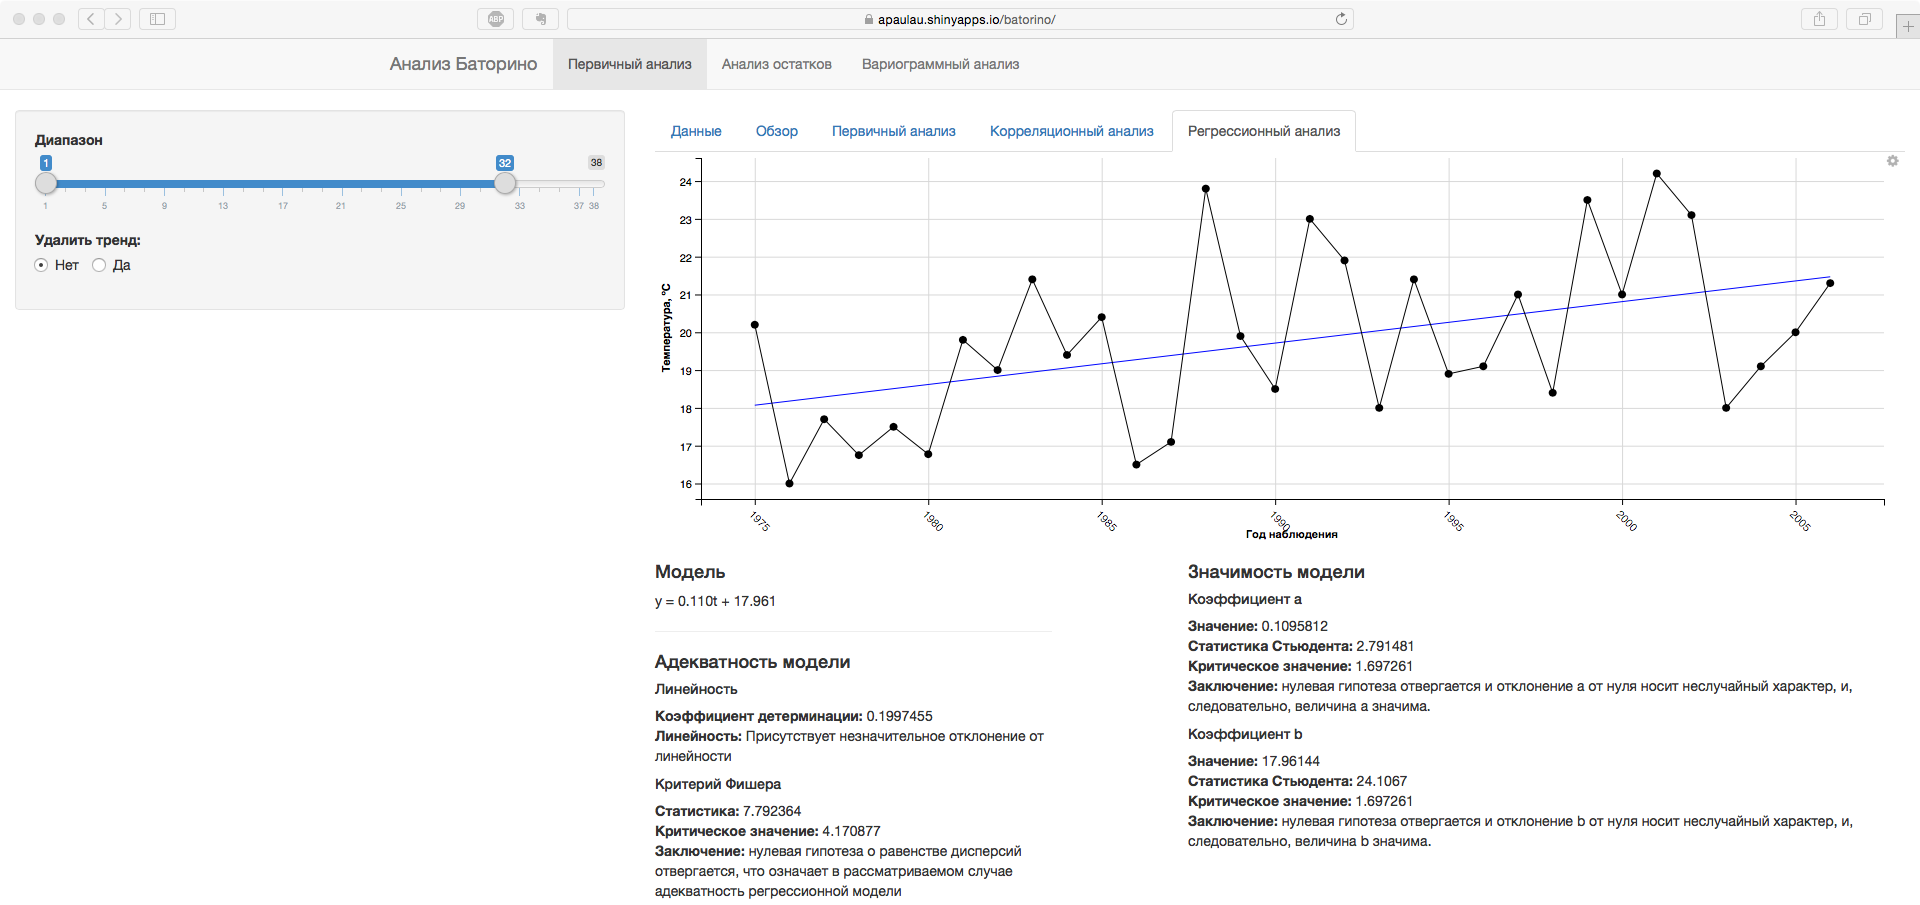
\includegraphics[width=0.75\textwidth]{../../figures/static/2_regr.png}
    \caption{Регрессионный анализ}
  \end{figure}
\end{frame}

\subsection{Модуль анализа остатков}

\begin{frame}
  % \frametitle{Автокорреляционная функция}
  \frametitle{Модуль анализа остатков}
    \begin{figure}[h]
    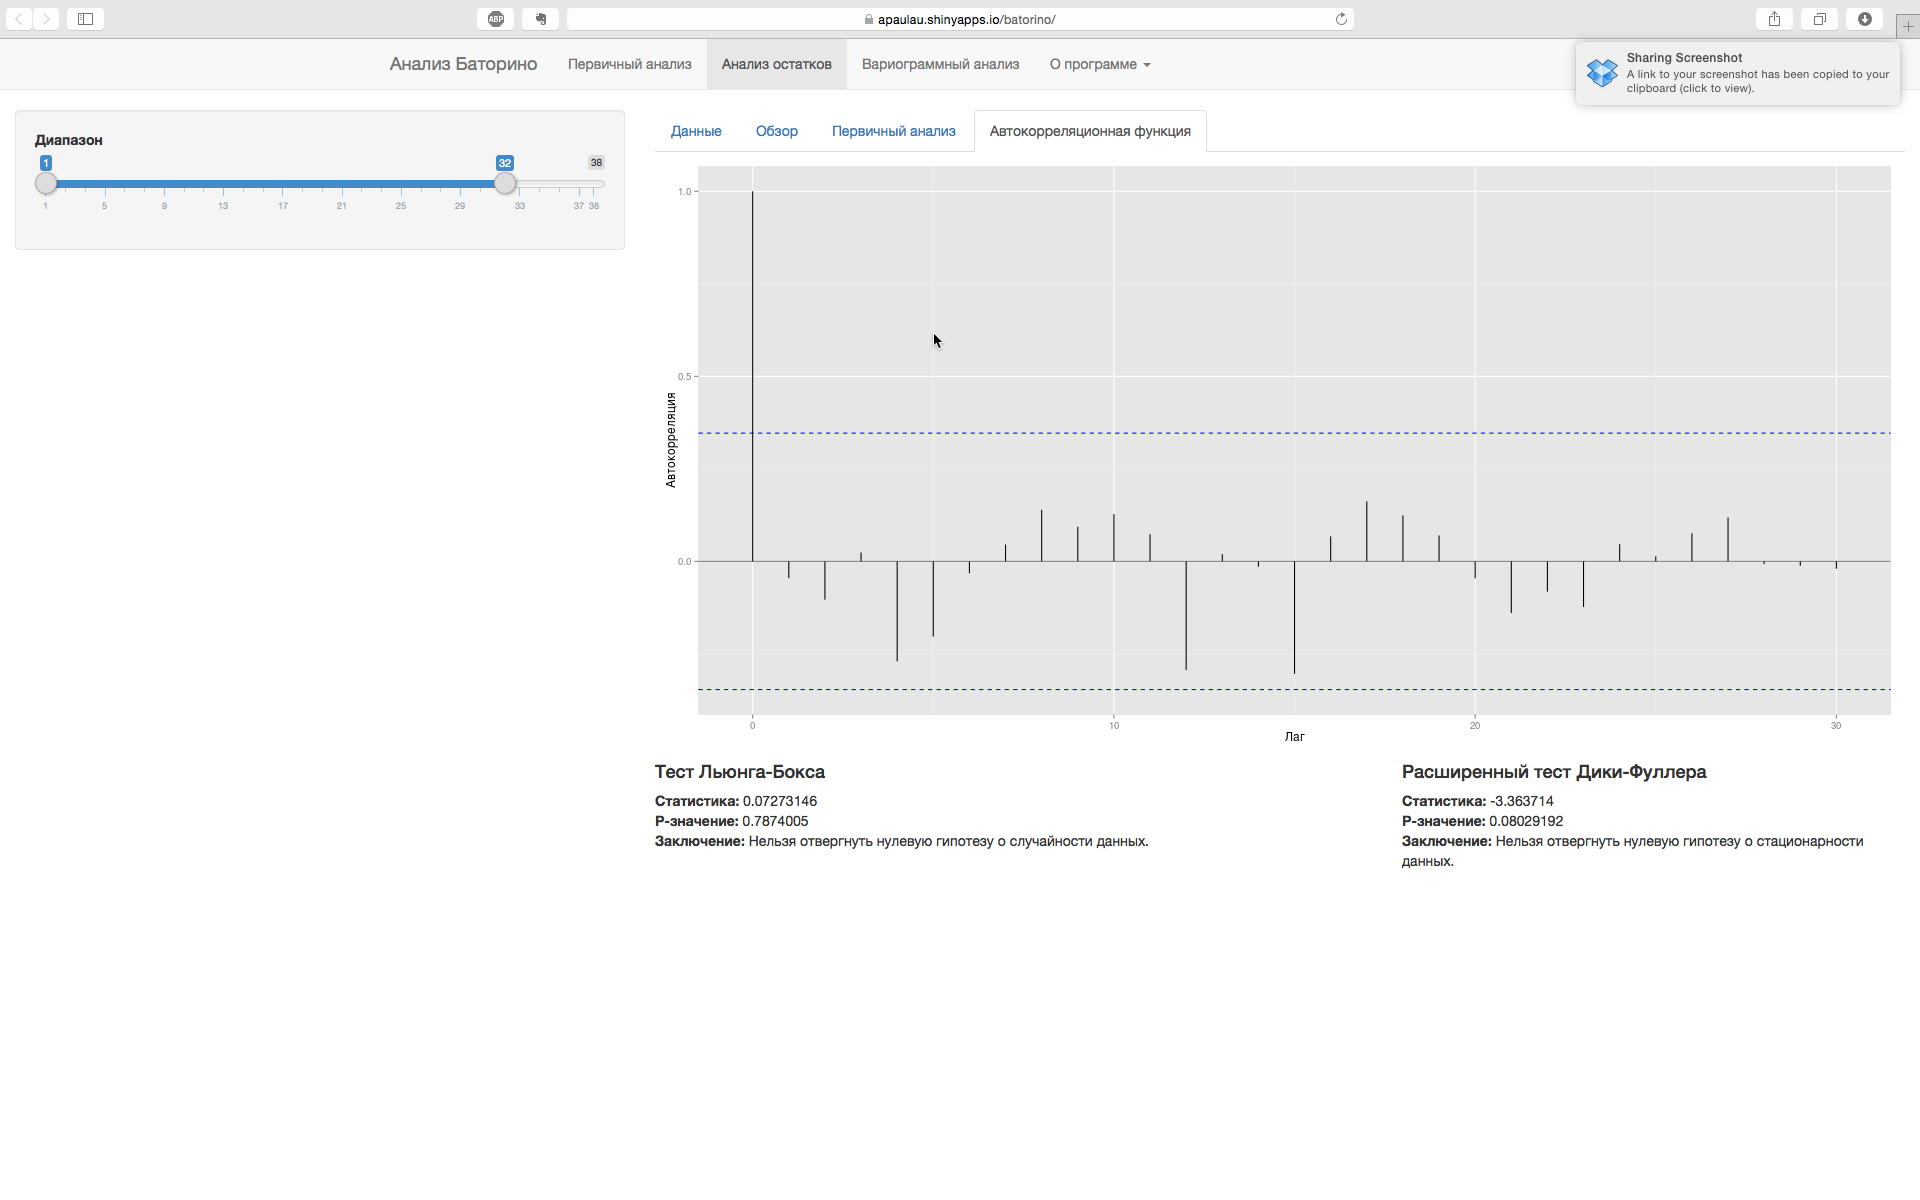
\includegraphics[width=0.75\textwidth]{../../figures/static/3_acf.png}
    \caption{Автокорреляционная функция}
  \end{figure}
\end{frame}

\subsection{Модуль вариограммного анализа}

\begin{frame}
  % \frametitle{Возможности по подбору модели вариограммы}
  \frametitle{Модуль вариограммного анализа}
    \begin{figure}[h]
    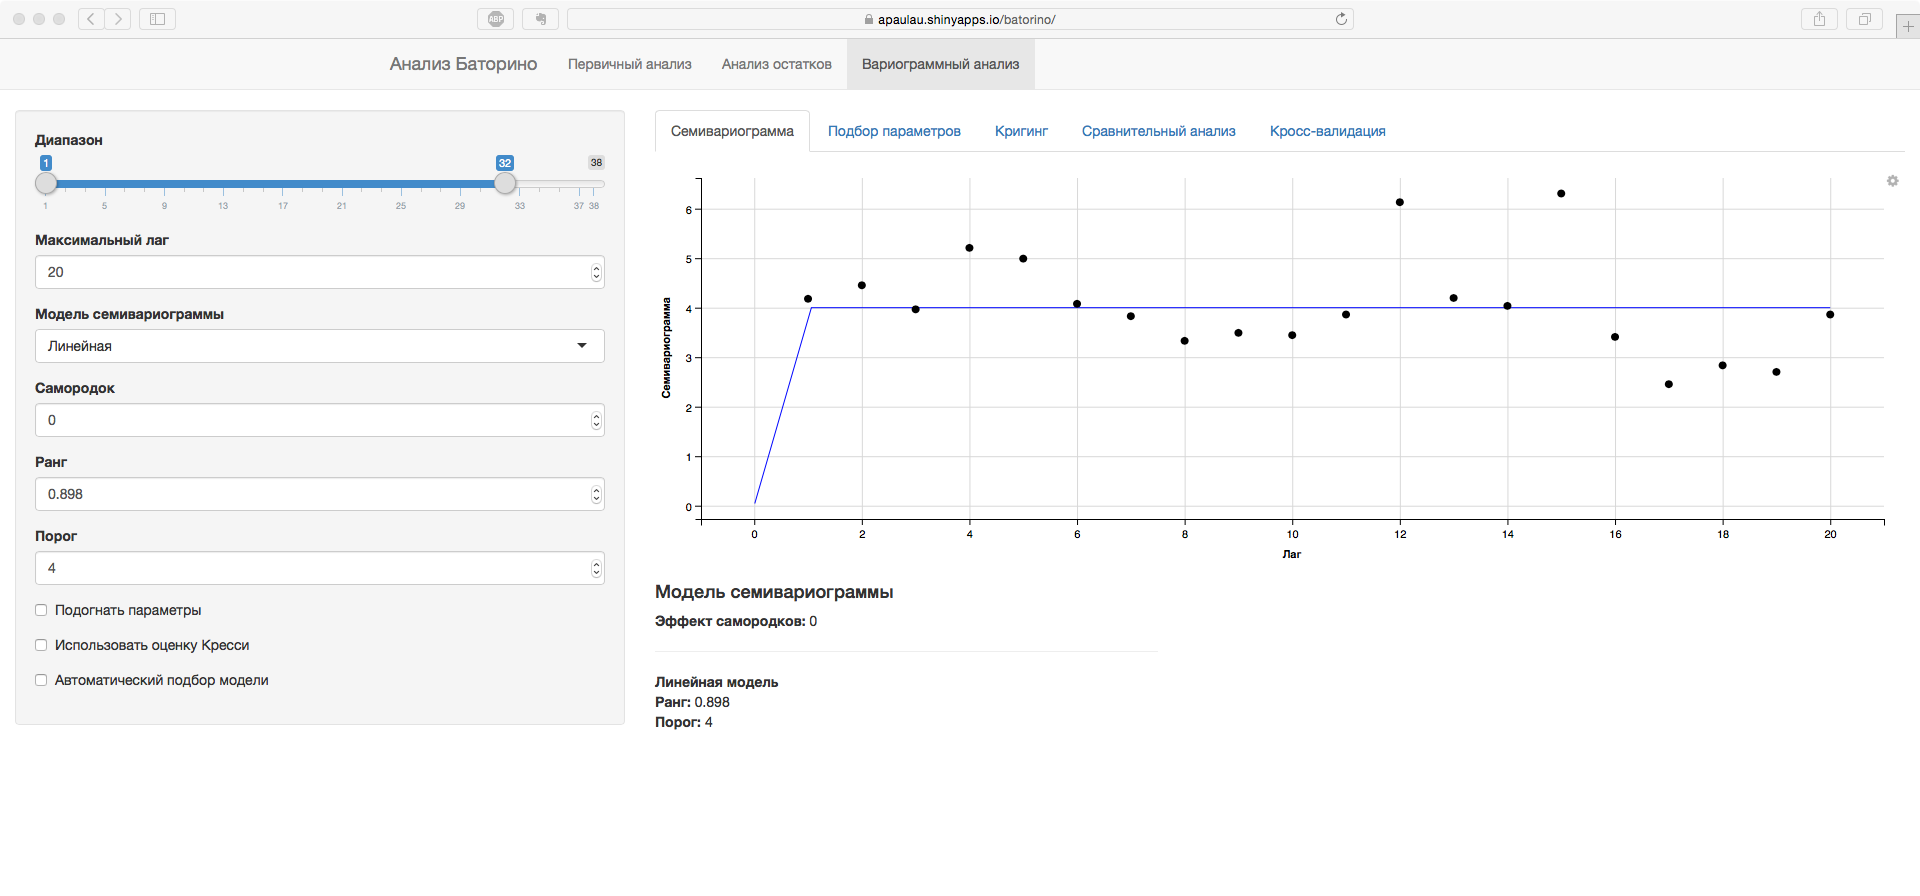
\includegraphics[width=0.75\textwidth]{../../figures/static/4_variogram.png}
    \caption{Возможности по подбору модели вариограммы}
  \end{figure}
\end{frame}

\begin{frame}
  % \frametitle{Подбор параметров модели вариограммы}
  \frametitle{Модуль вариограммного анализа}
    \begin{figure}[h]
    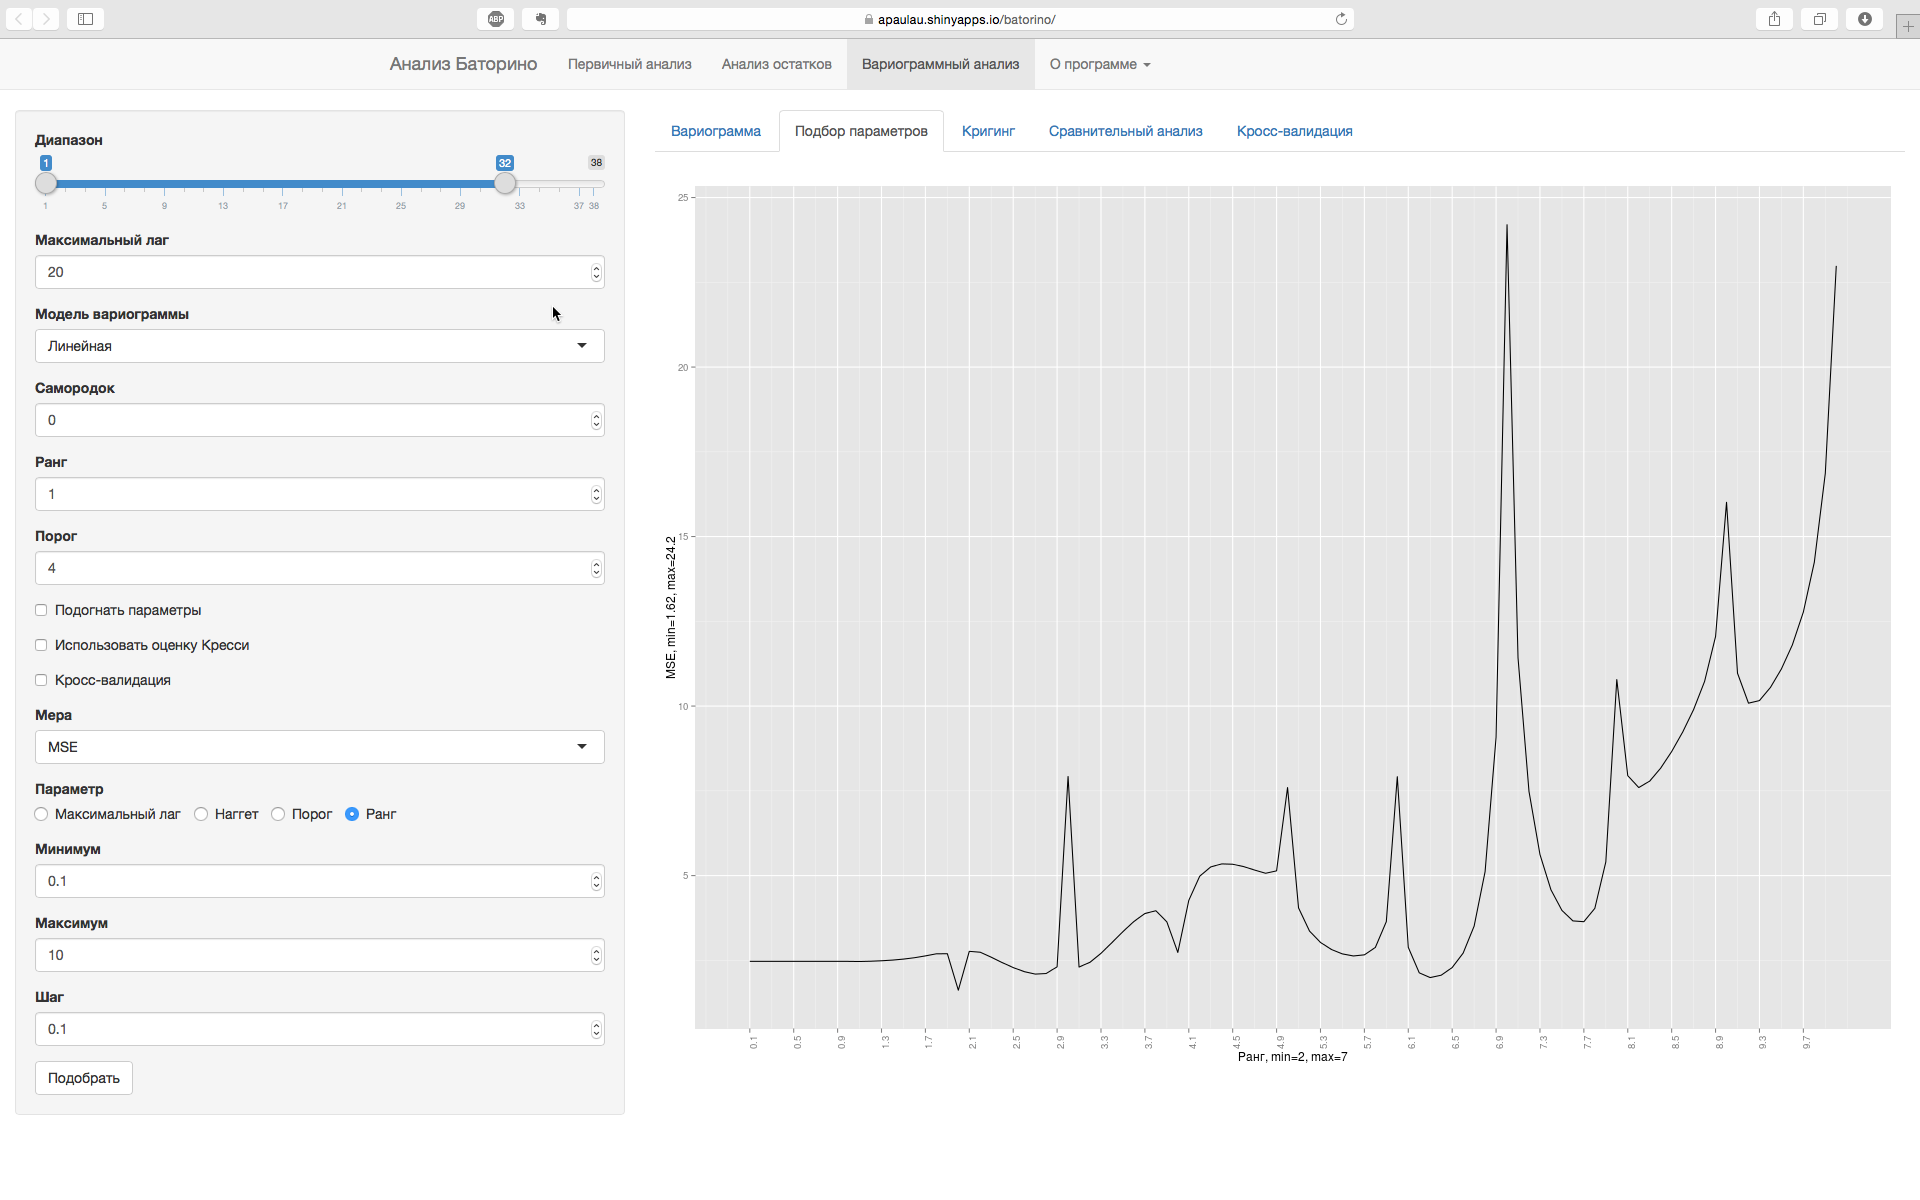
\includegraphics[width=0.75\textwidth]{../../figures/static/5_fit.png}
    \caption{Подбор параметров модели вариограммы}
  \end{figure}
\end{frame}

\begin{frame}
  % \frametitle{Сравнение прогнозных значений}
  \frametitle{Модуль вариограммного анализа}
    \begin{figure}[h]
    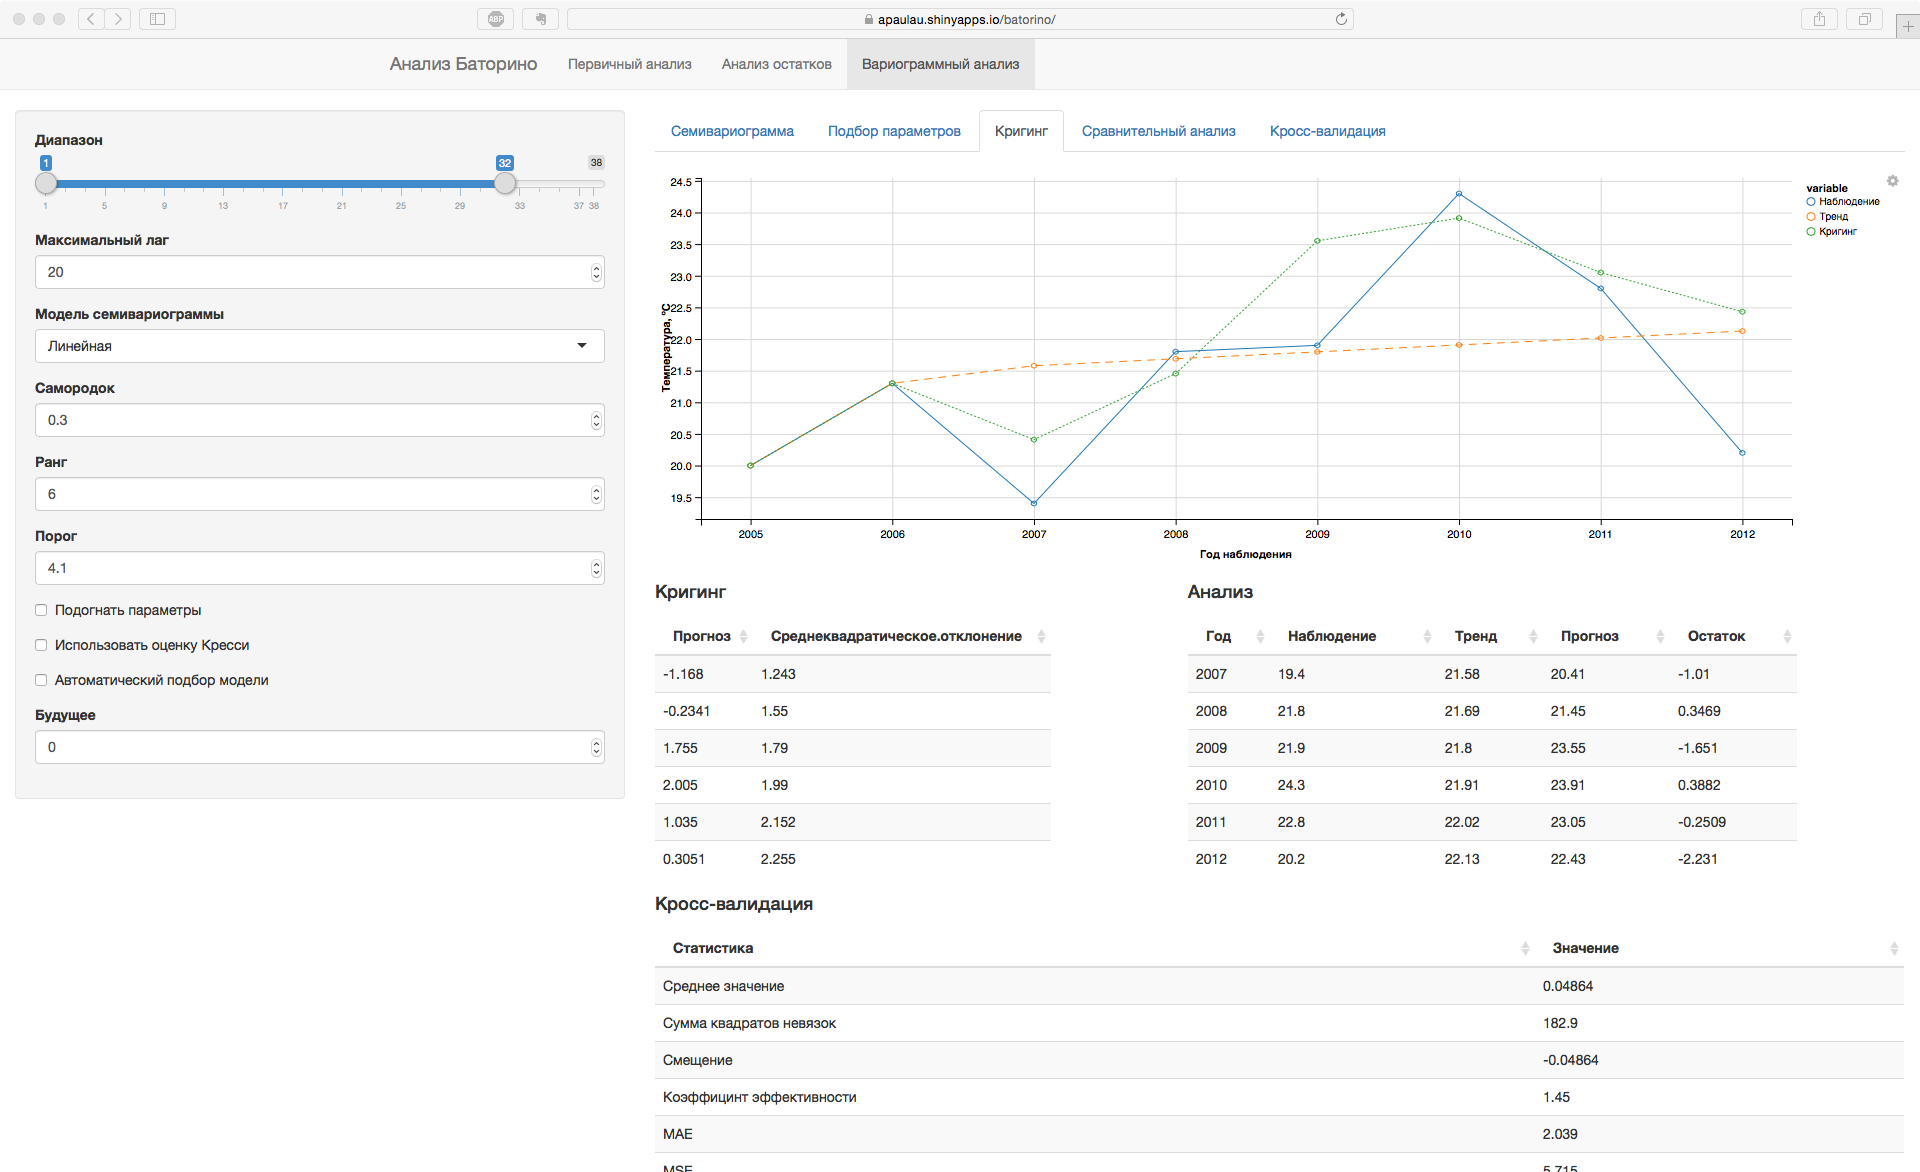
\includegraphics[width=0.75\textwidth]{../../figures/static/6_krige.png}
    \caption{Сравнение прогнозных значений}
  \end{figure}
\end{frame}

\section{Детерминированный подход}

\begin{frame}
  \frametitle{Исходные данные}
  \begin{columns}[c]
  \column{2in}
  Исседуемые данные получены от учебно-научного центра <<Нарочанская биологическая станция им. Г.Г.Винберга>>.

  Исходные данные представляют собой выборку $ X(t) $, состоящую из значений средней температуры воды в июле месяце каждый год в период с 1975 по 2012 годы.
  \column{4in}
  \begin{figure}[h]
    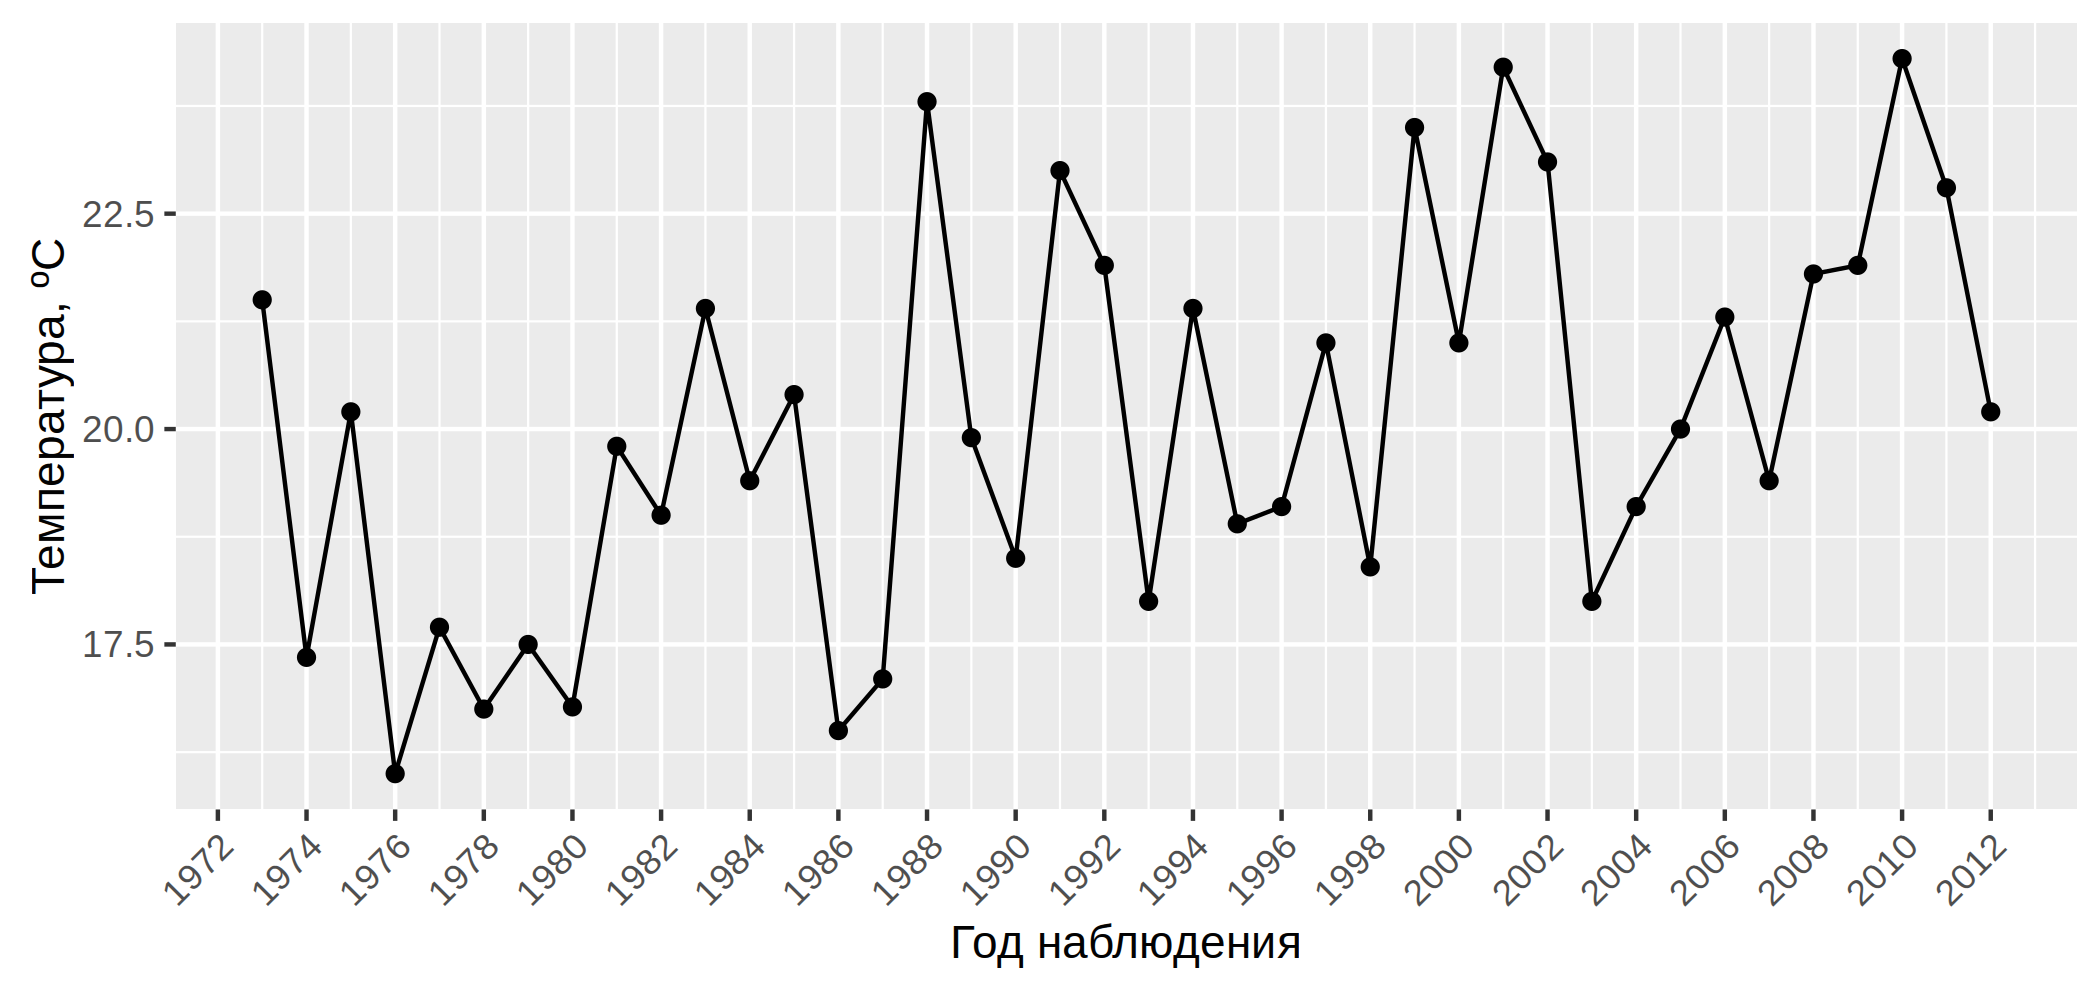
\includegraphics[width=1\linewidth]{../../figures/source.png}
    \caption{Исходные данные}
  \end{figure}
  \end{columns}
\end{frame}

\subsection{Проверка на нормальность}

\begin{frame}
  \frametitle{Проверка на нормальность}
  \begin{columns}[c]
  \column{2in}
  Визуально и проверкой критериев Шапиро-Уилка, $\chi^2$-Пирсона и Колмогороваа-Смирнова была показана близость выборочного распределения к нормальному с параметрами \normaldistr.

  При этом выборочное распредлеение характеризуется небольшой скошенностью вправо (коэффициент асимметрии $ \descriptive{original}{skew} $) и пологостью пика кривой распределения ($ \descriptive{original}{kurtosis} $) относительного нормального.
  \column{4in}
  \begin{figure}[h]
    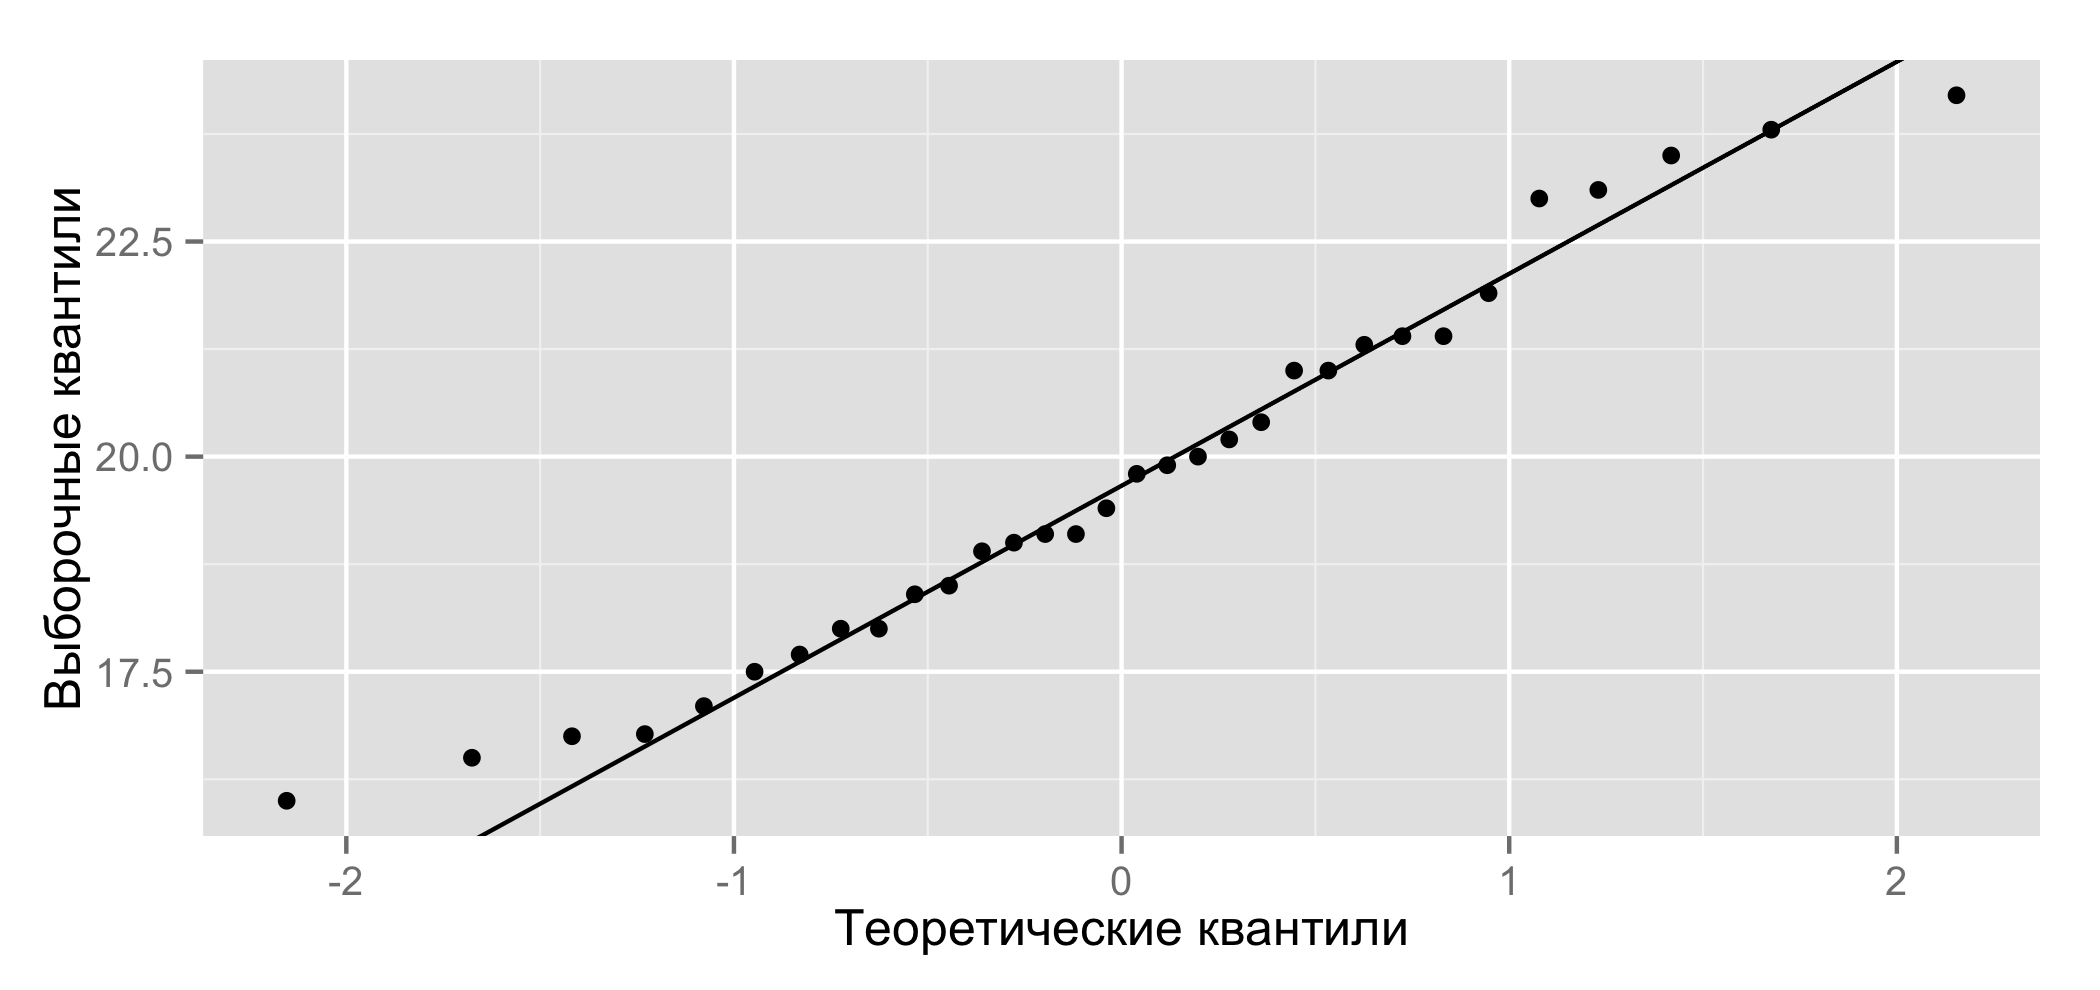
\includegraphics[width=1\linewidth]{../../figures/original/quantile.png}
    \caption{График квантилей}
  \end{figure}
  \end{columns}
\end{frame}

\subsection{Корреляционный анализ}

\begin{frame}
  \frametitle{Корреляционный анализ}
  \begin{columns}[c]
  \column{2in}
  С помощью критерия Граббса показано отсутствие выбросов в исходных данных.

  Вычислен выборочный коэффициент корреляции: $ r_{xt} = \characteristic{original}{correlation} $.

  При уровне значимости $ \alpha=0.05 $ доказана его значимость.
  \column{4in}
    \begin{figure}[h]
    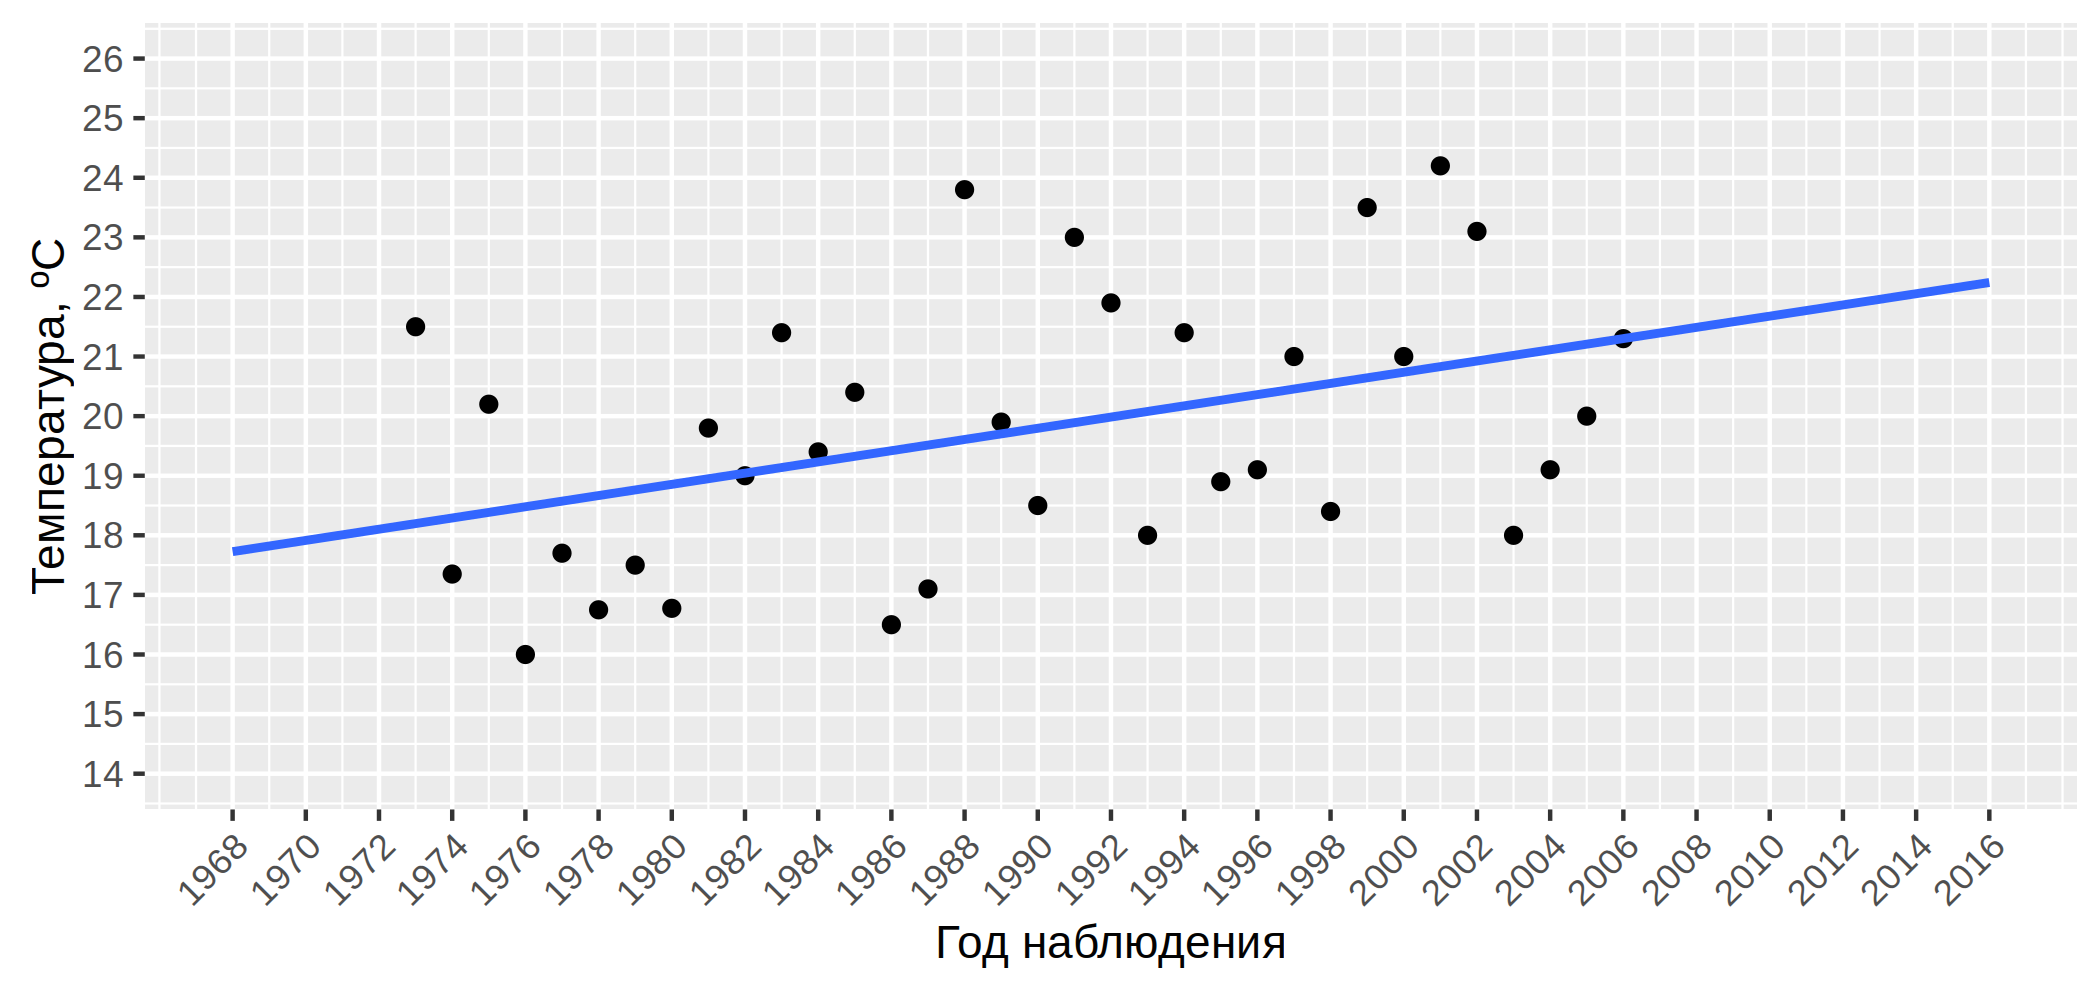
\includegraphics[width=1\linewidth]{../../figures/original/scatterplot.png}
    \caption{Диаграмма рассеяния}
  \end{figure}
  \end{columns}
\end{frame}

\subsection{Регрессионный анализ}

\subsubsection{Регрессионная модель}
\begin{frame}
  \frametitle{Регрессионная модель}
  \begin{columns}[c]
  \column{2in}
  Выявлено, что исследуемый временной ряд является аддитивным:
  \begin{equation}
    X(t) = y(t) + \varepsilon(t),
  \end{equation}
  где $ y(t) $ --- тренд, $ \varepsilon(t) $ --- нерегулярная составляющая.
  Найдена модель тренда: $ y(t) = at + b = 0.1014t + 18.0521 $
  \column{4in}
    \begin{figure}[h]
    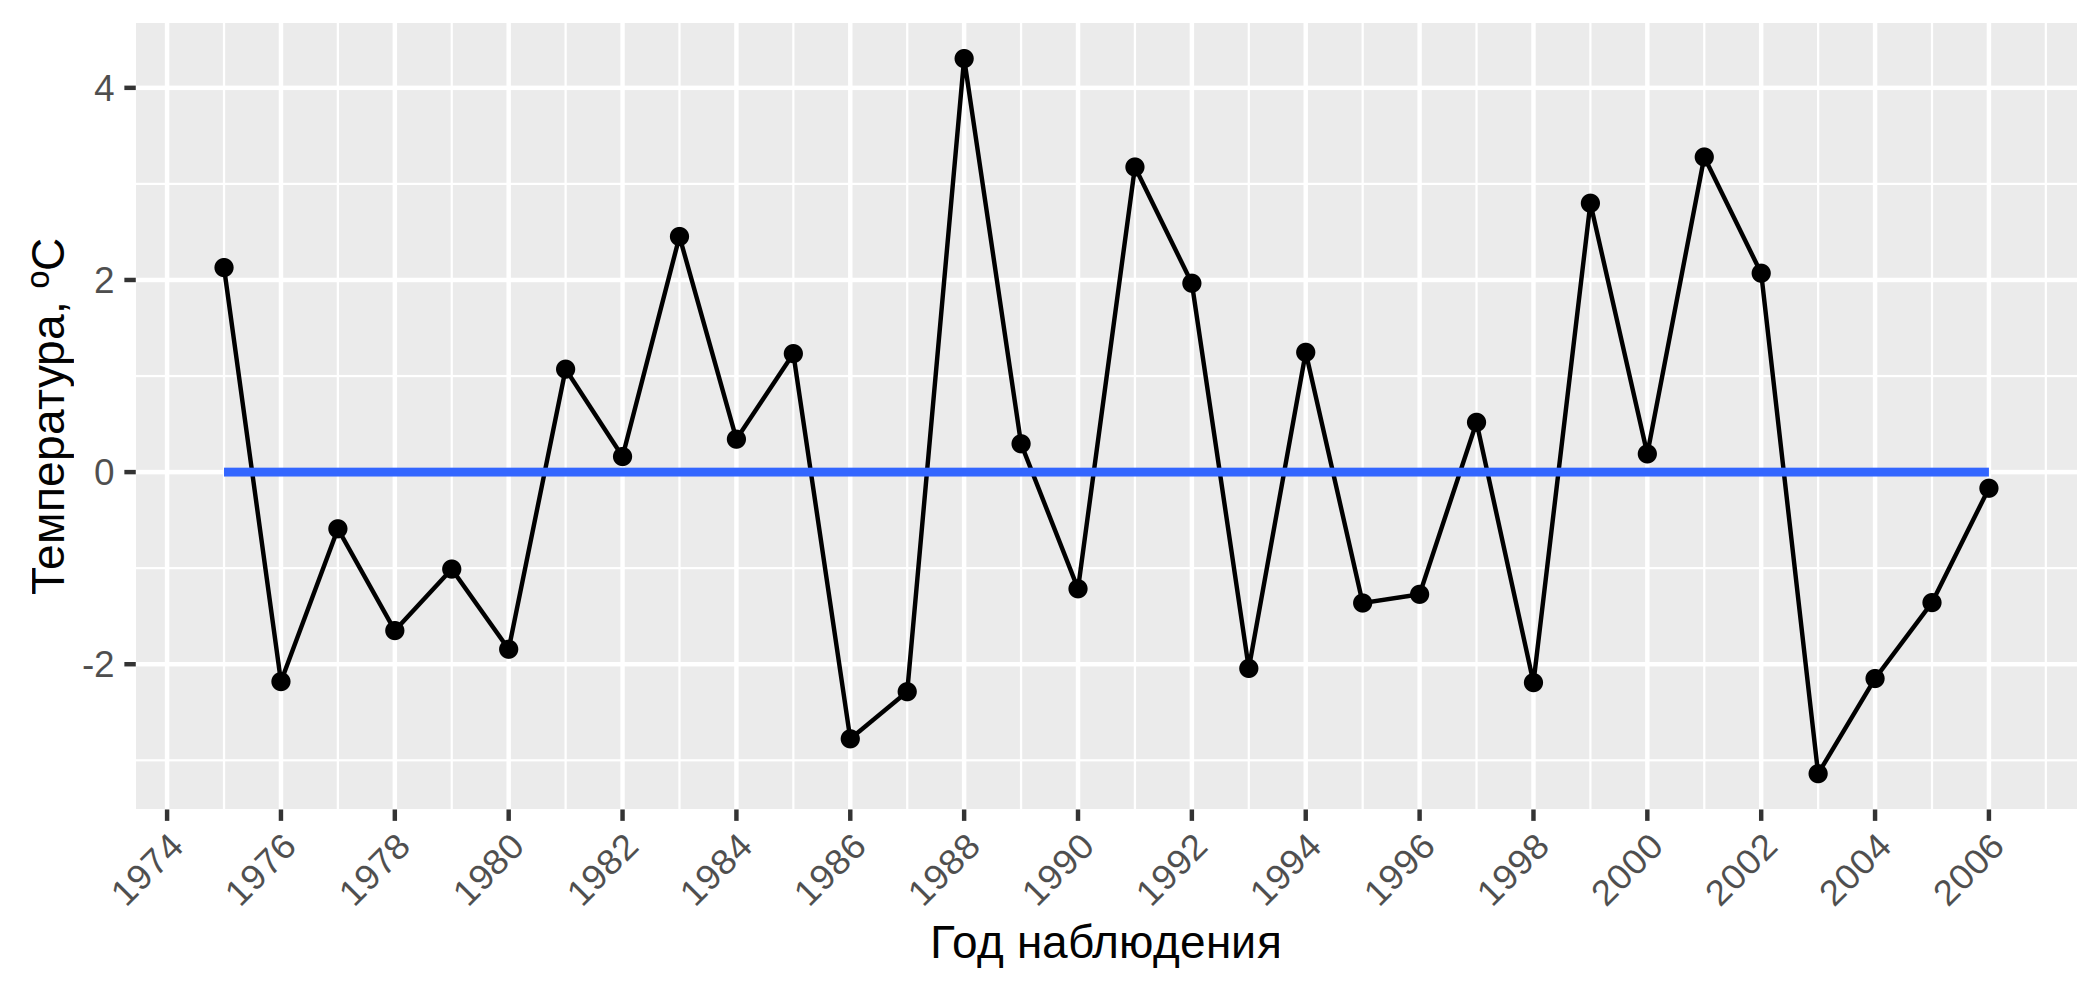
\includegraphics[width=1\linewidth]{../../figures/residual/time-series.png}
    \caption{Ряд остатков $ \varepsilon(t) $}
  \end{figure}
  \end{columns}
\end{frame}

\subsubsection{Качество регрессионной модели}
\begin{frame}
  \frametitle{Оценка модели}
  \begin{itemize}
    \item С помощью критерия Стьюдента, при уровне значимости $ \alpha=0.05 $, доказана значимость коэффициентов регрессионной модели
    \item F-критерий Фишера при уровне значимости $ \alpha = 0.05 $ показал адекватность модели
    \item Точность модели невысока, поскольку коэффициент детерминации $ \eta^2_{x(t)} = 0.275 $
  \end{itemize}
\end{frame}

\subsection{Анализ остатков}
\begin{frame}[shrink=9]
  \frametitle{Анализ остатков}
  \begin{columns}[c]
  \column{2.2in}
    Визуально и проверкой тестов показана близость выборочного распределения к нормальному \resnormaldistr.

    На графике видно, что значения автокорреляций не выходят за интервал, обозначенный пунктиром. Что значит отсутствие значимых автокорреляций. Проведённый тест подтвердил данное замечание.

    Также было отмечено, что значения имеют небольшую амплитуду и затухают с ростом лага. Это говорит о стационарности в широком смысле, что подтвердил расширенный тест Дики-Фуллера.
  \column{4.2in}
    \begin{figure}[h]
    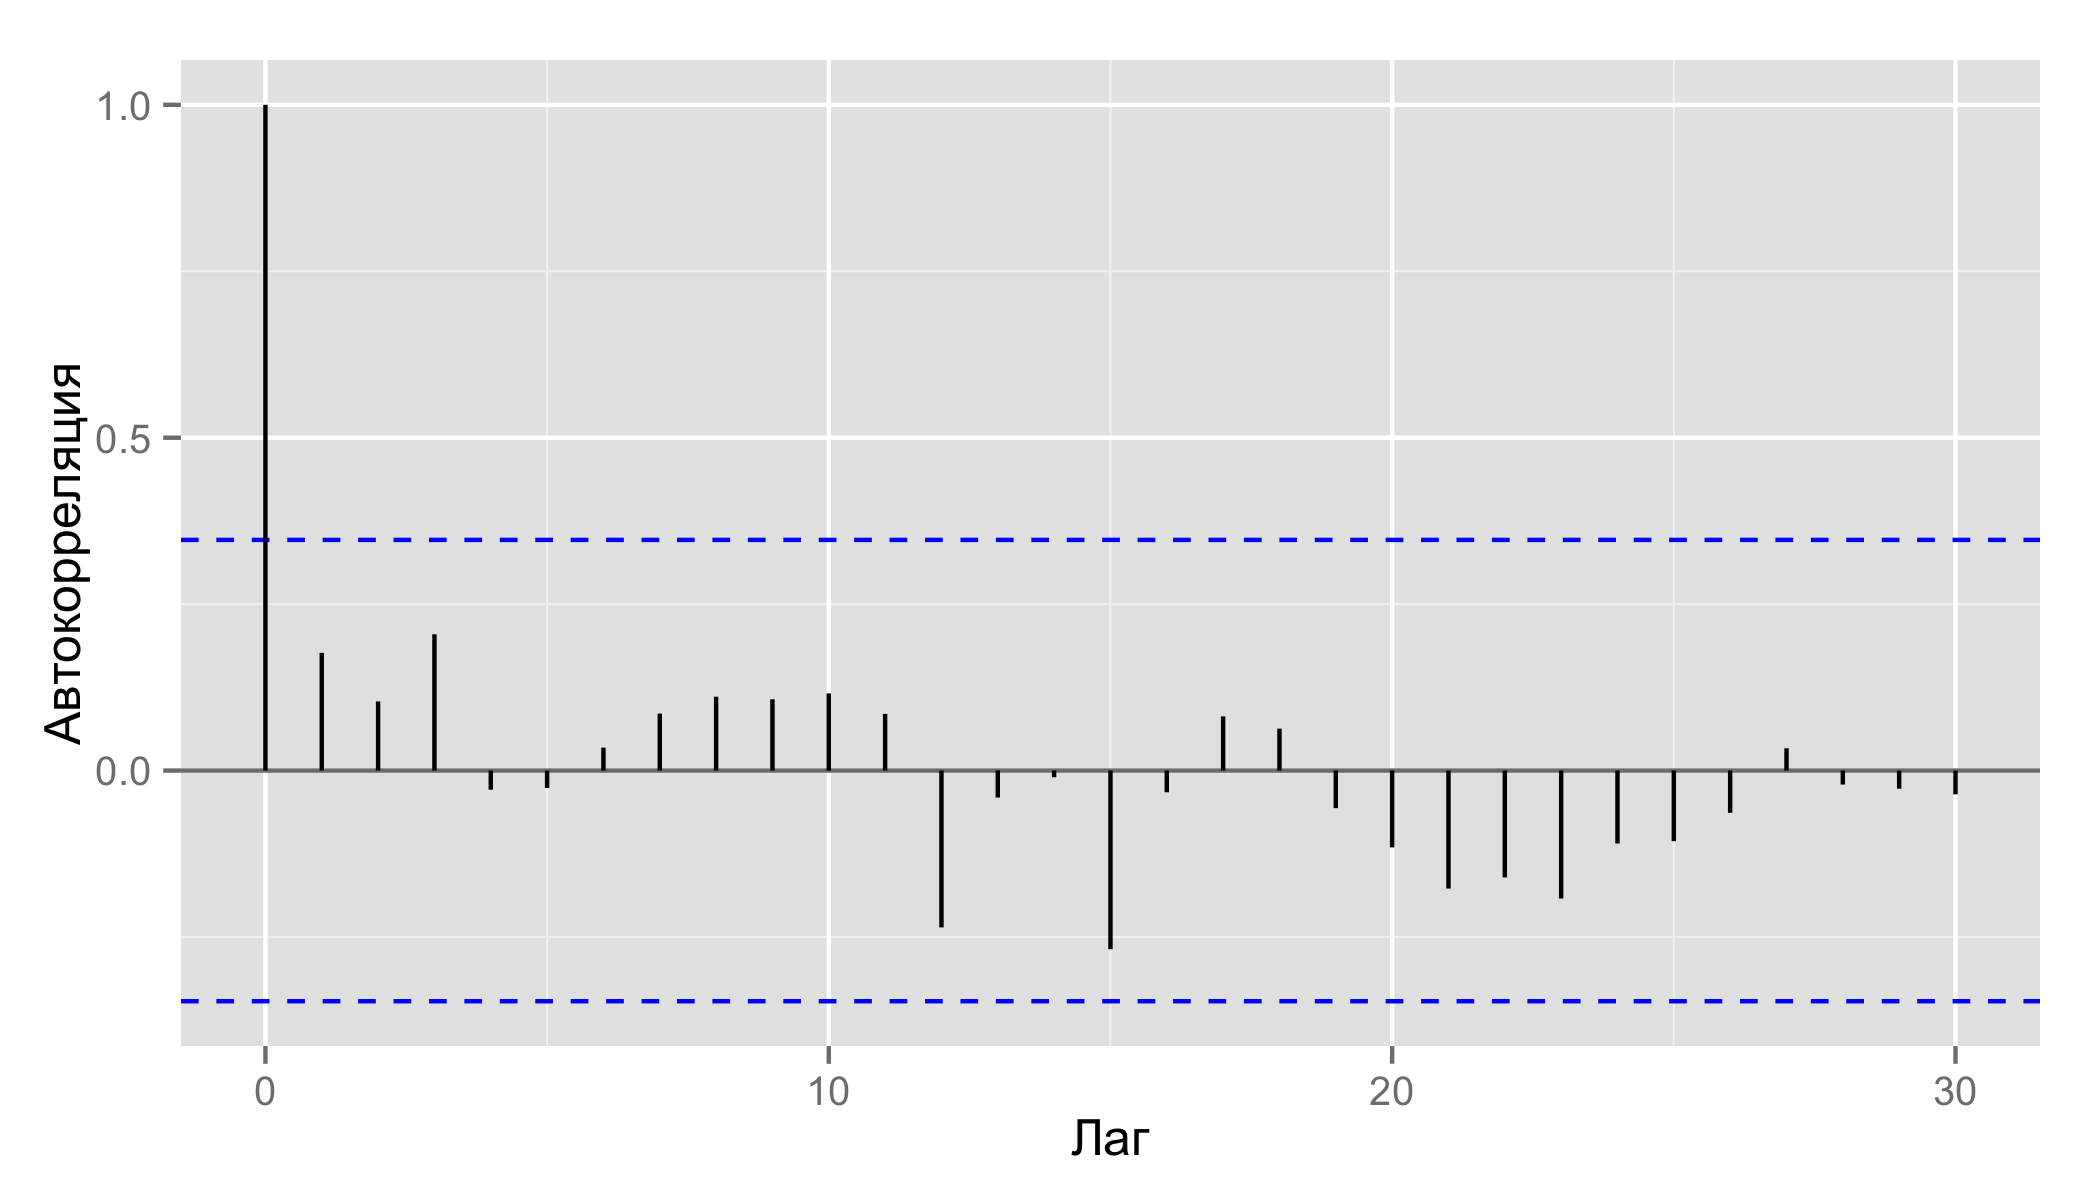
\includegraphics[width=1\linewidth]{../../figures/residual/acf.png}
    \caption{Автокорреляционная функция}
  \end{figure}
  \end{columns}
\end{frame}

\section{Геостатистический подход}

\subsection{Введение}

\begin{frame}
  \frametitle{Оценка вариограммы}
  Рассмотривается стационарный в широком смысле гауссовский случайный процесс с дискретным временем $ X(t),~ t \in \mathbb{Z} $, нулевым математическим ожиданием, постоянной дисперсией и неизвестной вариограммой $ 2 \gamma(h), h \in \mathbb{Z} $.
  \begin{Definition}
    \textit{Вариограммой} случайного процесса $ X(t), t \in \mathbb{Z} $, называется функция вида
    \begin{equation}
        2 \gamma (h) = V \{ X(t + h) - X(t) \},~ t, h \in \mathbb{Z}.
    \end{equation}

    При этом функция $ \gamma (h), h \in \mathbb{Z} $, называется \textit{семивариограммой}.
  \end{Definition}
  В качестве оценки вариограммы рассматривается статистика, предложенная Матероном:
  \begin{equation}
    2 \tilde{\gamma}(h) = \frac{1}{n - h} \sum_{t = 1}^{n - h}(X(t + h) - X(t))^2, \quad h = \overline{0, n - 1},
  \end{equation}
\end{frame}

\begin{frame}
  \frametitle{Первые два момента оценки вариограммы}
\begin{Theorem}
  Для оценки $ 2 \tilde{\gamma}(h) $ имеют место следующие соотношения:
  \begin{equation*}
    E \{2 \tilde{\gamma}(h) \} = 2 \gamma(h), % DIRTY HACK
  \end{equation*}
  \begin{equation*}
    cov(2 \tilde{\gamma}(h_1), 2 \tilde{\gamma}(h_2)) =
  \end{equation*}
  \begin{equation*}
    = \frac{2}{(n - h_1)(n - h_2)} \sum_{t = 1}^{n - h_1}\sum_{s = 1}^{n - h_2} (\gamma(t - h_2 - s) + \gamma(t + h_1 - s) - \gamma(t - s) - \gamma(t + h_1 - s - h_2))^2,
  \end{equation*}
  \begin{equation*}
    V \{ 2 \tilde{\gamma}(h) \} = \frac{2}{(n-h)^2}\sum_{t,s = 1}^{n - h} ( \gamma(t - h - s) + \gamma(t + h - s) - 2\gamma(t - s) )^2,
  \end{equation*}
  где $ \gamma(h), h \in \mathbb{Z} $, --- семивариограмма процесса $ X(t), t \in \mathbb{Z}$, $ h, h_1, h_2 = \overline{0, n - 1} $.
\end{Theorem}
\end{frame}

\begin{frame}
  \frametitle{Асимптотическое поведение оценки вариограммы}
  \begin{Theorem}
  Если имеет место соотношение
  \begin{equation*}
    \sum_{h = -\infty}^{+\infty} \vert \gamma(h) \vert < +\infty, \text{то}
  \end{equation*}
  \begin{equation*}
    \lim_{n \to \infty} (n - \min\{ h_1, h_2 \}) cov\{ 2 \tilde{\gamma}(h_1), 2 \tilde{\gamma}(h_2) \} = 2 \sum_{m = -\infty}^{+\infty} \gamma(m - h_2) + \gamma(m + h_1) - \gamma(m) - \gamma(m + h_1 - h_2))^2,
  \end{equation*}
  \begin{equation*}
    \lim_{n \to \infty} (n - h) V\{ 2 \tilde{\gamma}(h) \} = 2 \sum_{m = -\infty}^{+\infty} \gamma(m - h) + \gamma(m + h) - 2 \gamma(m))^2.
  \end{equation*}
  где $ \gamma(h), h \in \mathbb{Z} $, --- семивариограмма процесса $ X(t), t \in \mathbb{Z}$, $ h, h_1, h_2 = \overline{0, n - 1} $.
\end{Theorem}
\end{frame}

\subsection{Вариограммный анализ}

\begin{frame}
  \frametitle{График экспериментальной вариограммы}
   \begin{columns}[c]
   \column{4.5in}
  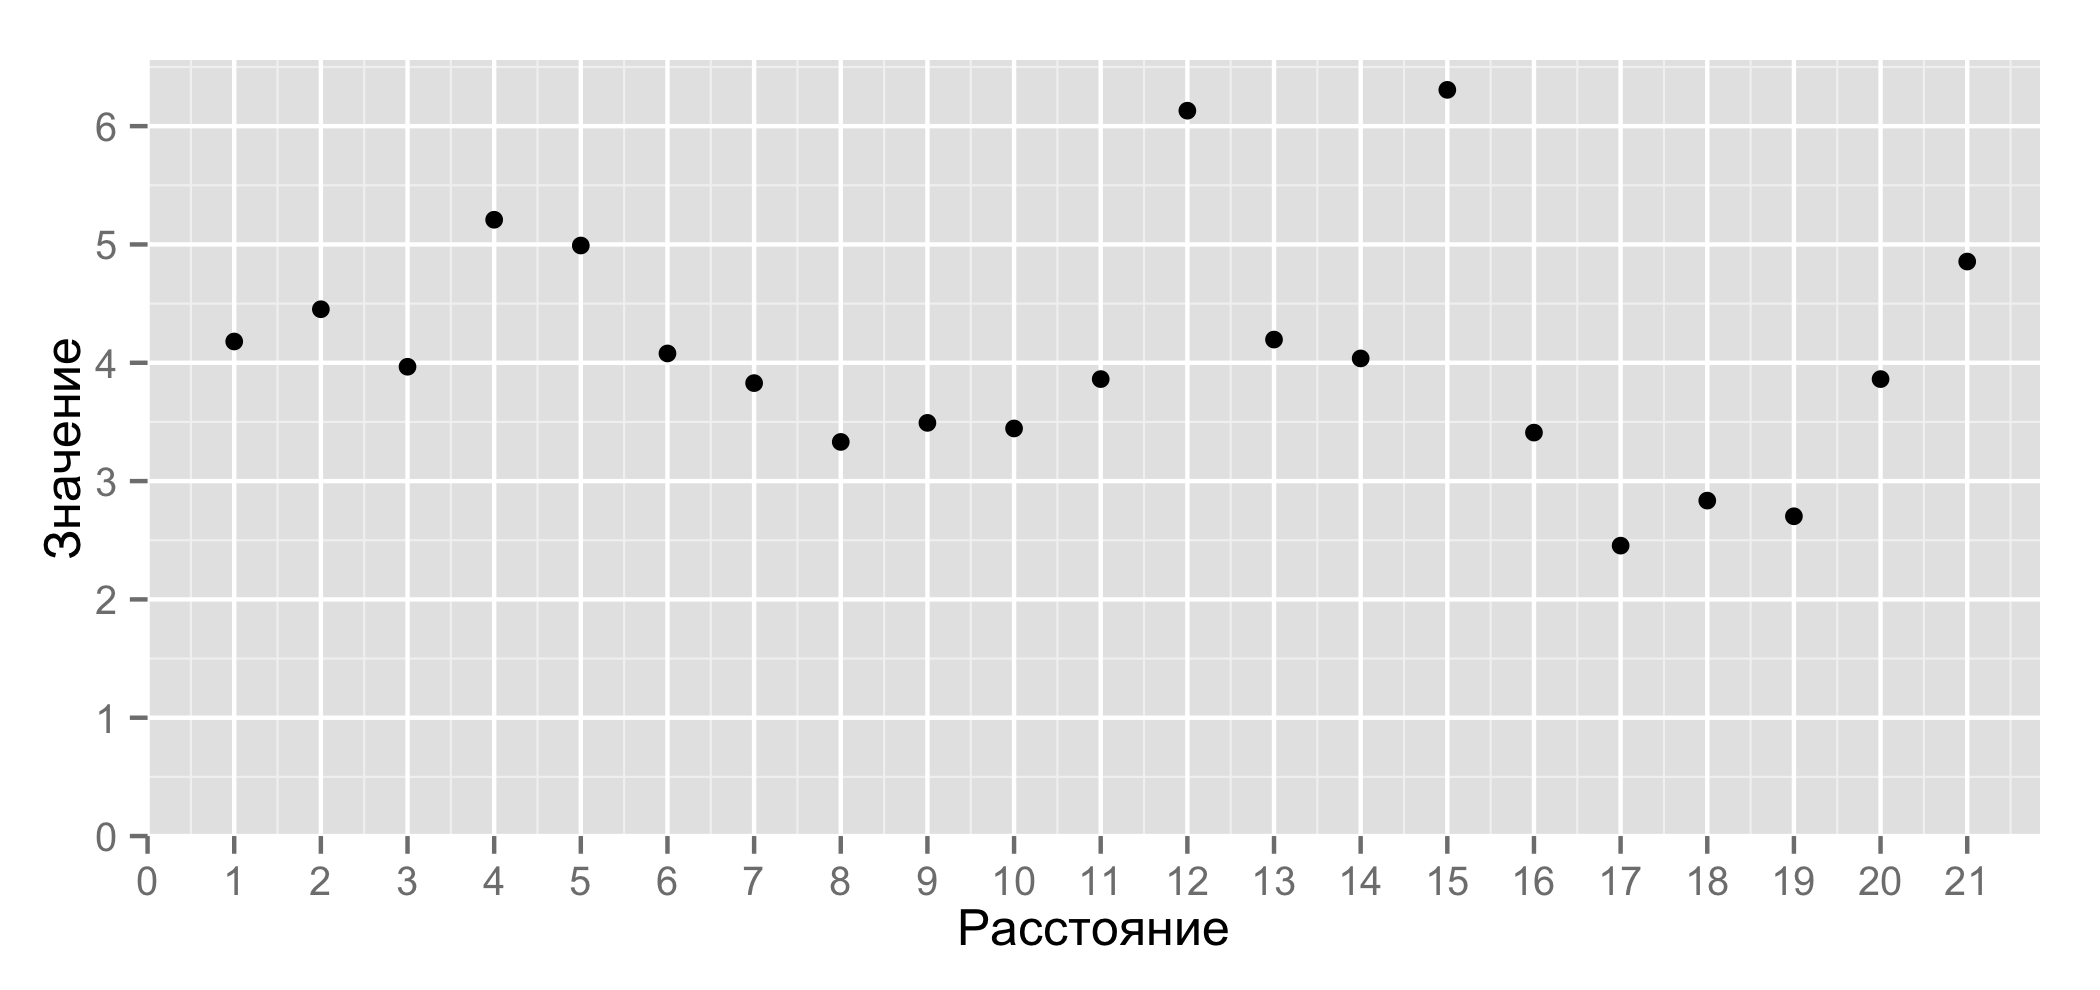
\includegraphics[width=0.95\textwidth]{../../figures/variogram/lin-variogram.png}
  \end{columns}
\end{frame}

\begin{frame}
  \frametitle{Линейная модель с порогом}
  \begin{columns}[c]
  \column{2in}
  Подобранная модель: $ 0.3 + 4 \cdot Lin(h, 6.2) $
  \column{3in}
   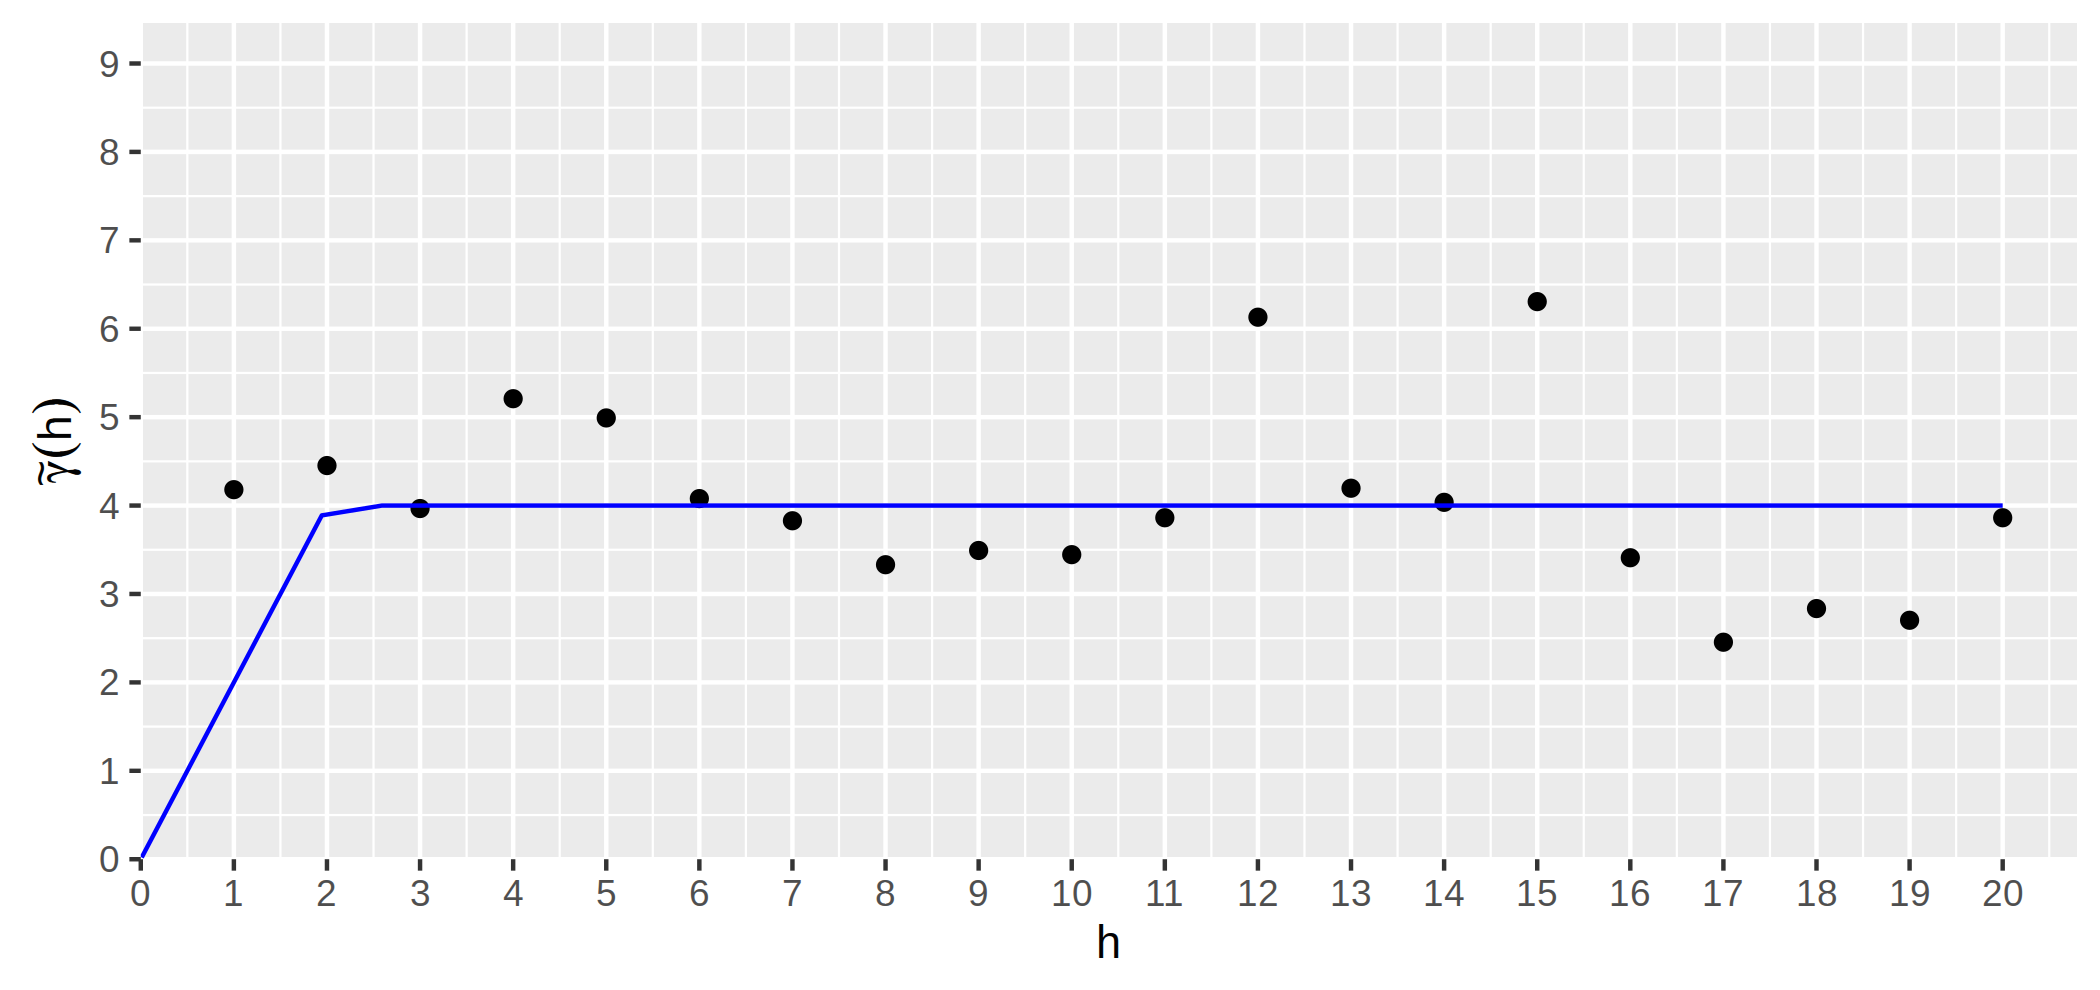
\includegraphics[width=3in]{../../figures/variogram/lin-fit-adapt-modeled.png}
  \end{columns}
\end{frame}

\subsection{Кригинг}
\begin{frame}
  \frametitle{Прогнозирование методом ординарного кригинга}
  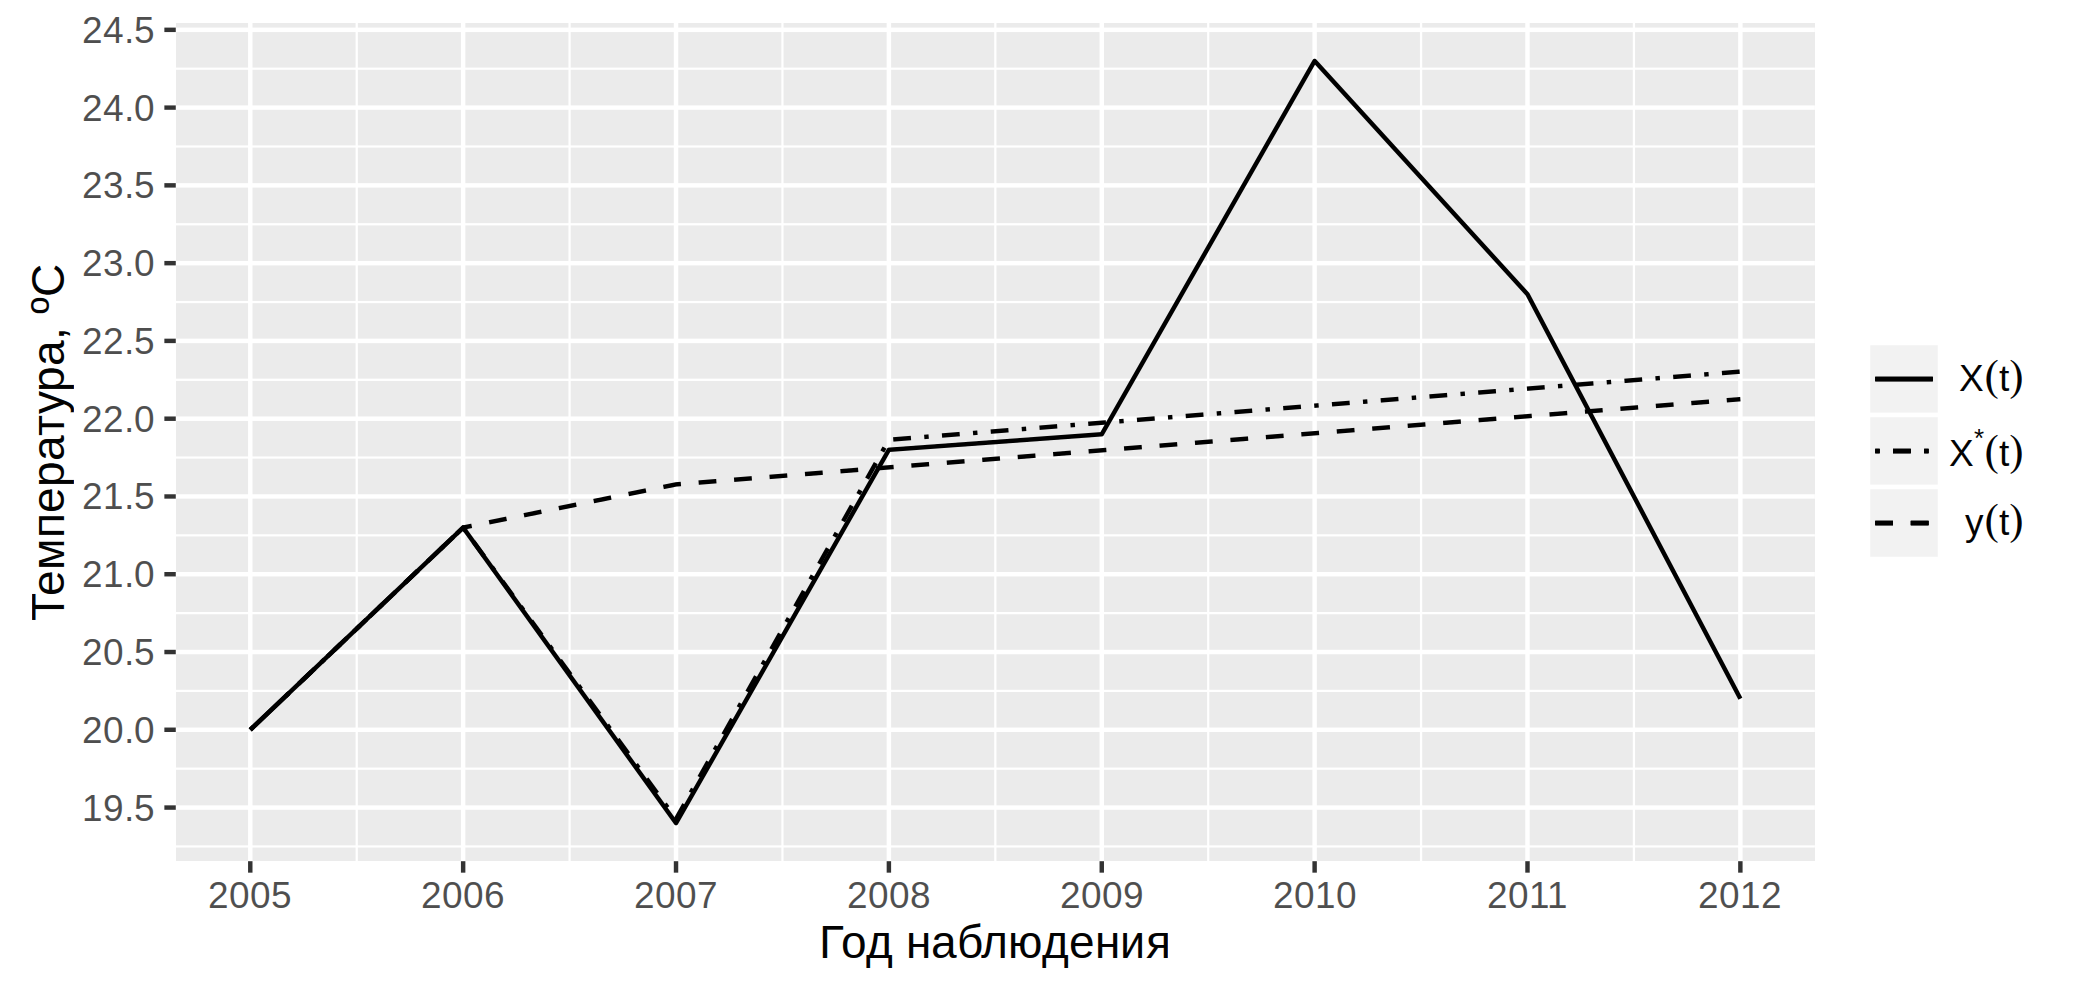
\includegraphics[width=0.95\textwidth]{../../figures/variogram/lin-fit-adapt-cross-prediction.png}
\end{frame}

\begin{frame}
  \frametitle{Периодическая модель}
  \begin{columns}[c]
  \column{2in}
  Подобранная модель: $ 4 \cdot Per(h, 0.898) $
  \column{3in}
   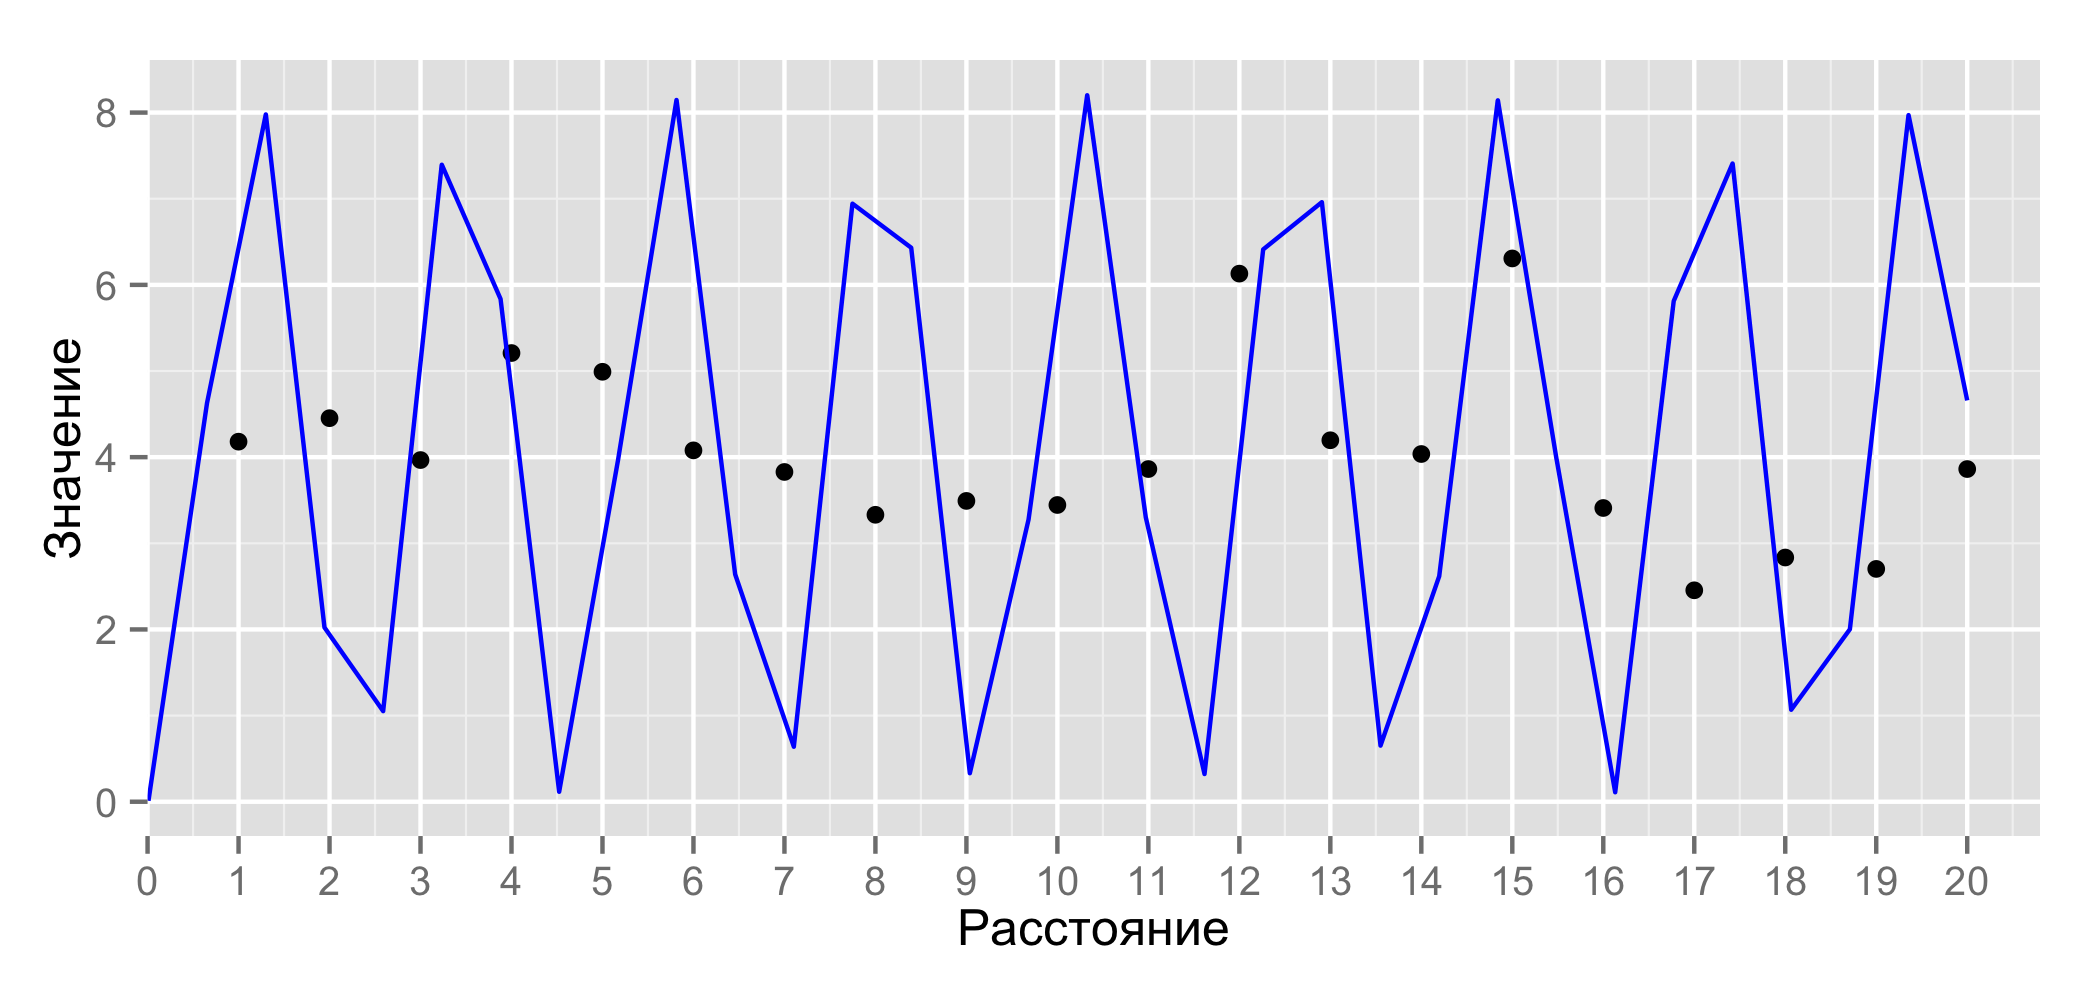
\includegraphics[width=3in]{../../figures/variogram/per-fit-cv-modeled.png}
  \end{columns}
\end{frame}

\begin{frame}
  \frametitle{Прогнозирование методом ординарного кригинга}
  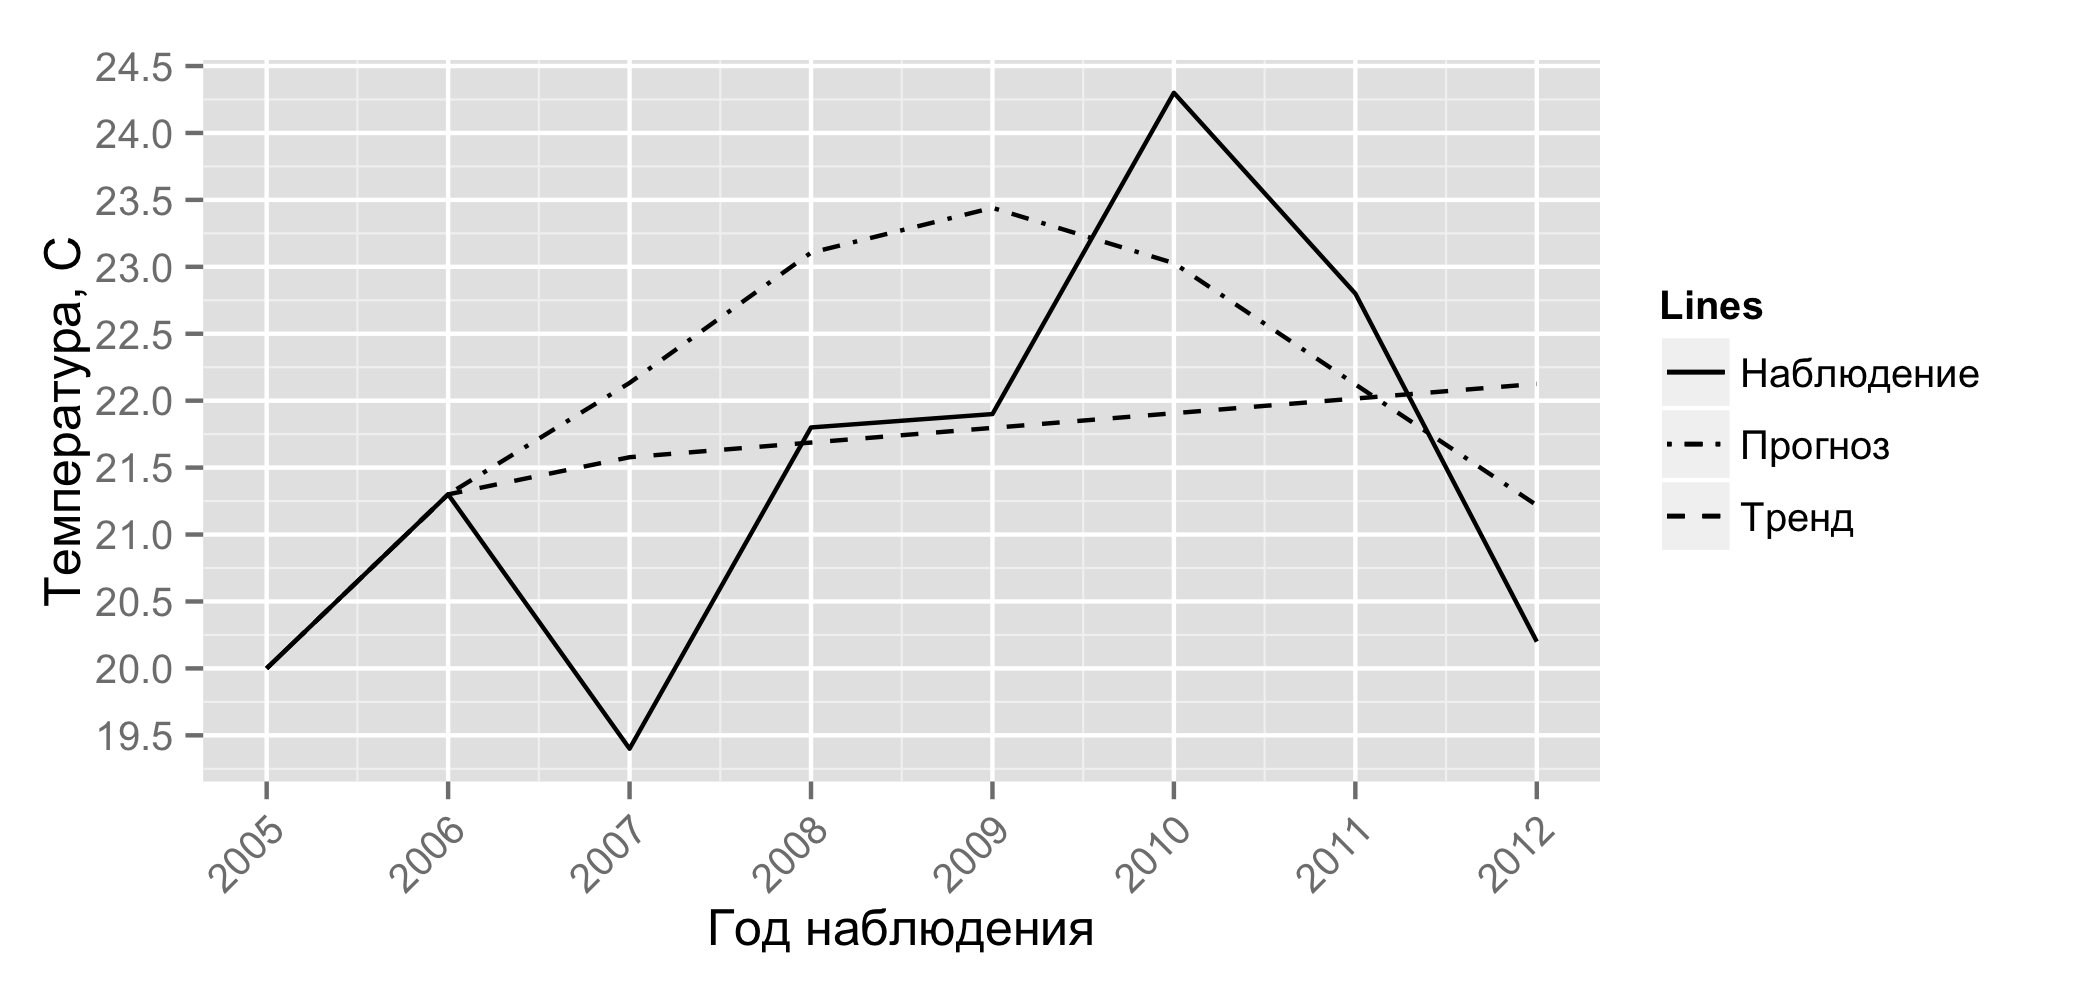
\includegraphics[width=0.95\textwidth]{../../figures/variogram/per-fit-cv-cross-prediction.png}
\end{frame}

\subsection{Автоматический подбор}

\begin{frame}
  \frametitle{Периодическая модель}
  \begin{columns}[c]
  \column{2in}
  Подобранная модель: $ 3.8 + 0.32 \cdot Per(h, 1.3) $
  \column{3in}
   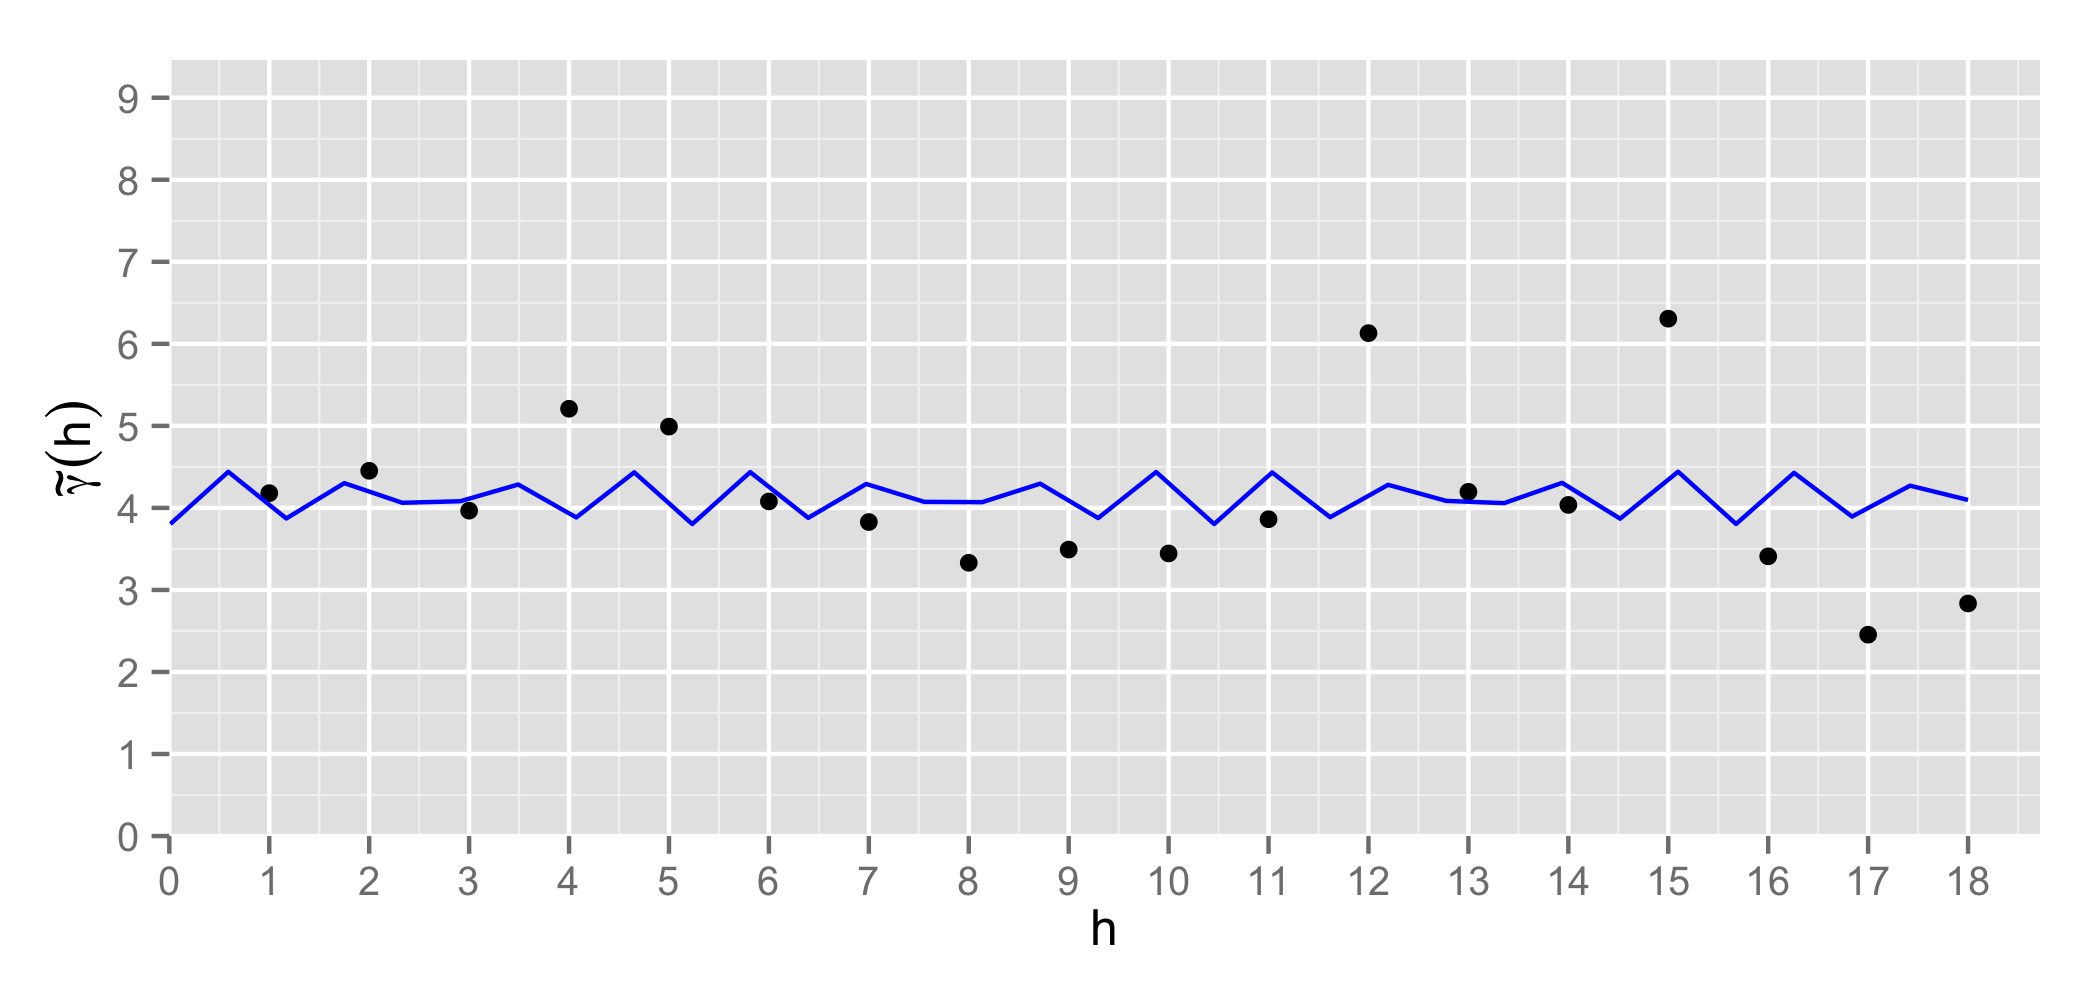
\includegraphics[width=3in]{../../figures/variogram/auto-class-18-modeled.png}
  \end{columns}
\end{frame}

\begin{frame}
  \frametitle{Прогнозирование методом ординарного кригинга}
  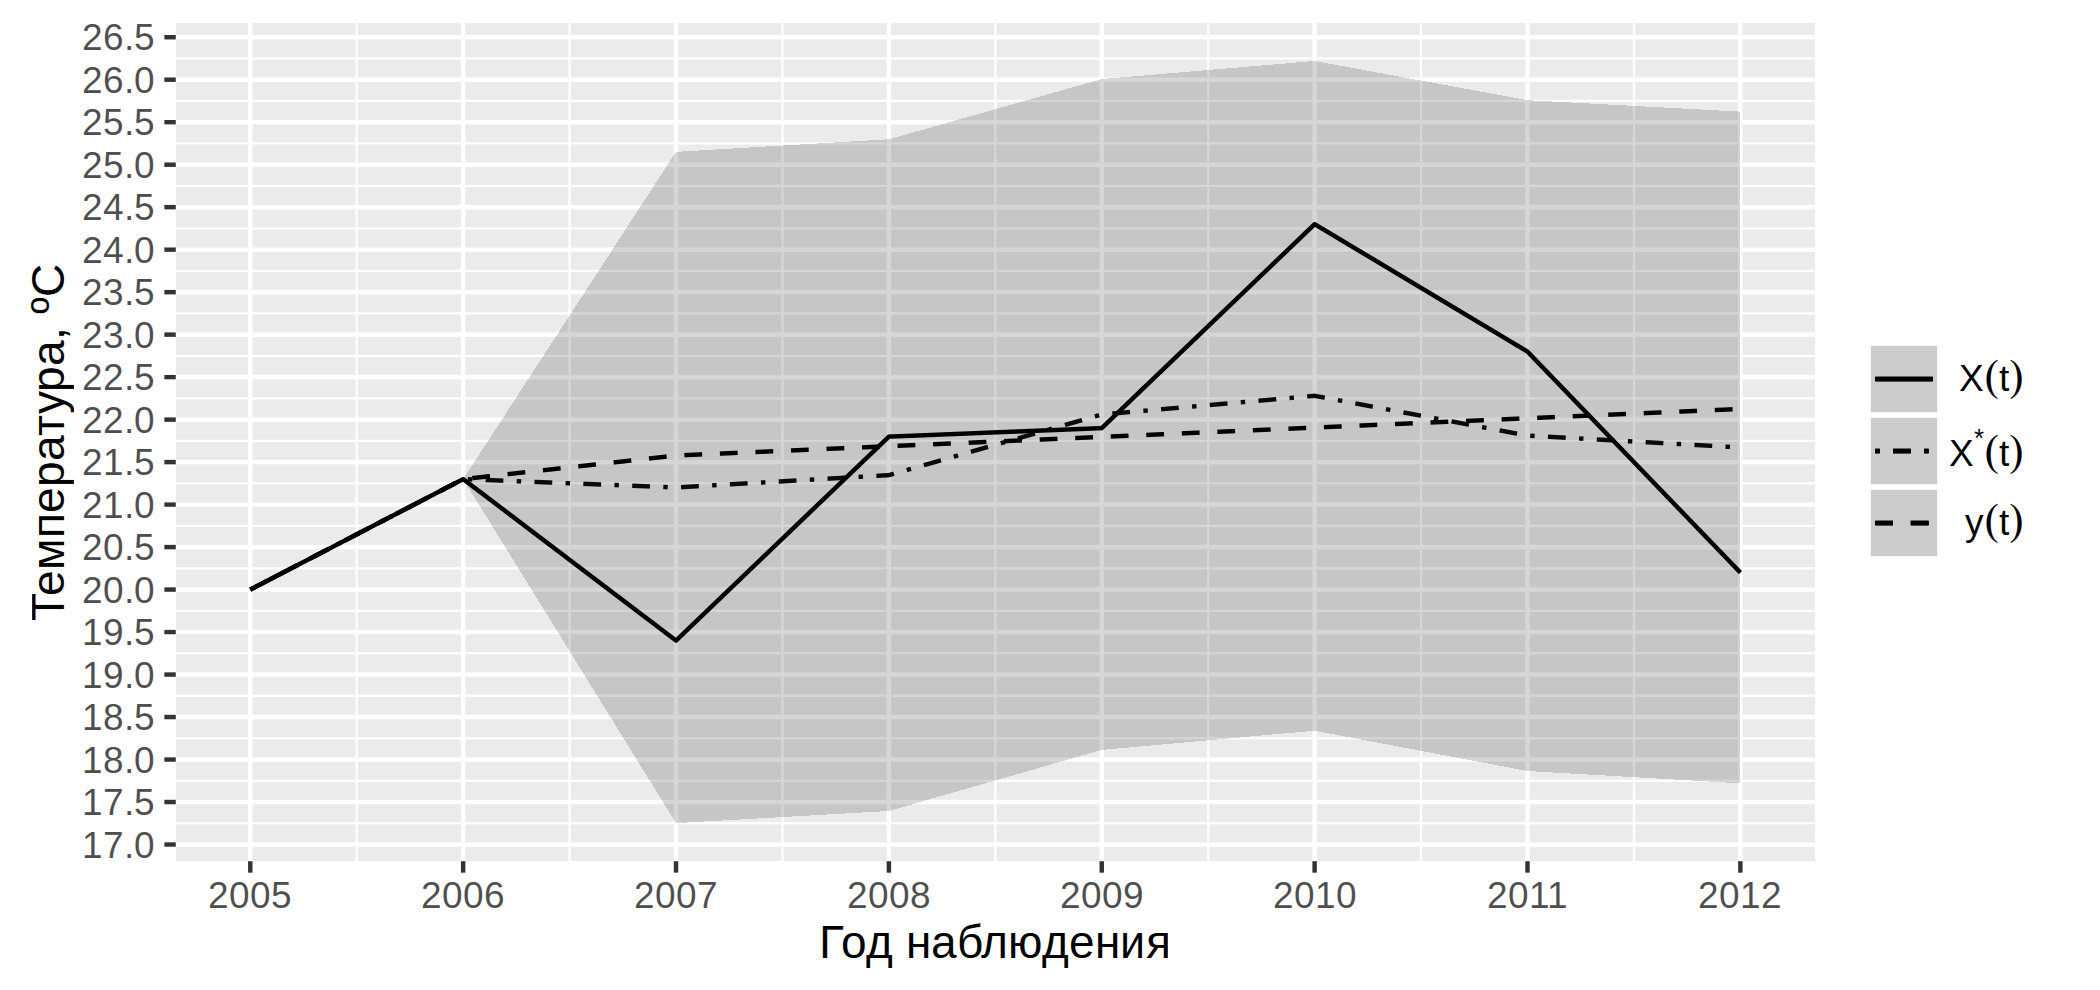
\includegraphics[width=0.95\textwidth]{../../figures/variogram/auto-class-18-cross-prediction.png}
\end{frame}

\begin{frame}
  \frametitle{Волновая модель}
  \begin{columns}[c]
  \column{2in}
  Подобранная модель: $ 4.11 + 1.65 \cdot Wav(h, 3.59) $
  \column{3in}
   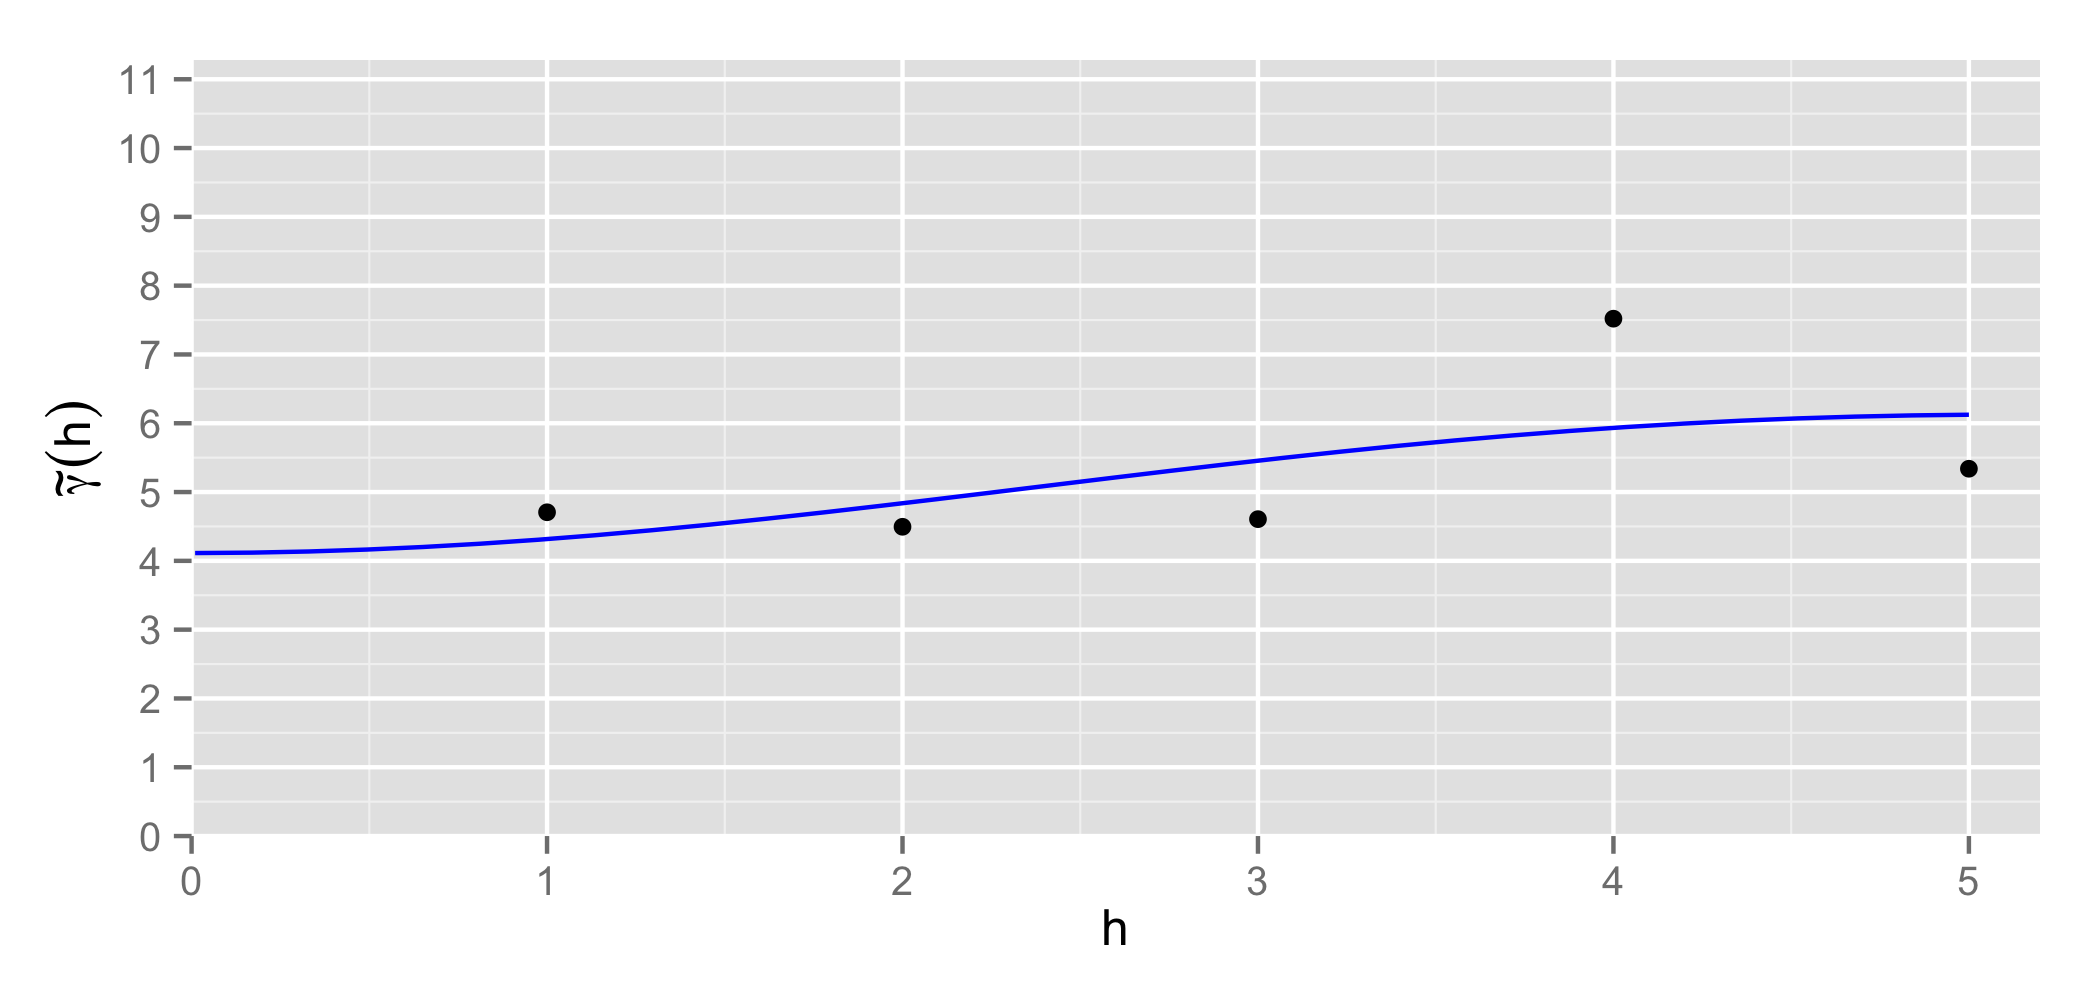
\includegraphics[width=3in]{../../figures/variogram/auto-rob-5-modeled.png}
  \end{columns}
\end{frame}

\begin{frame}
  \frametitle{Прогнозирование методом ординарного кригинга}
  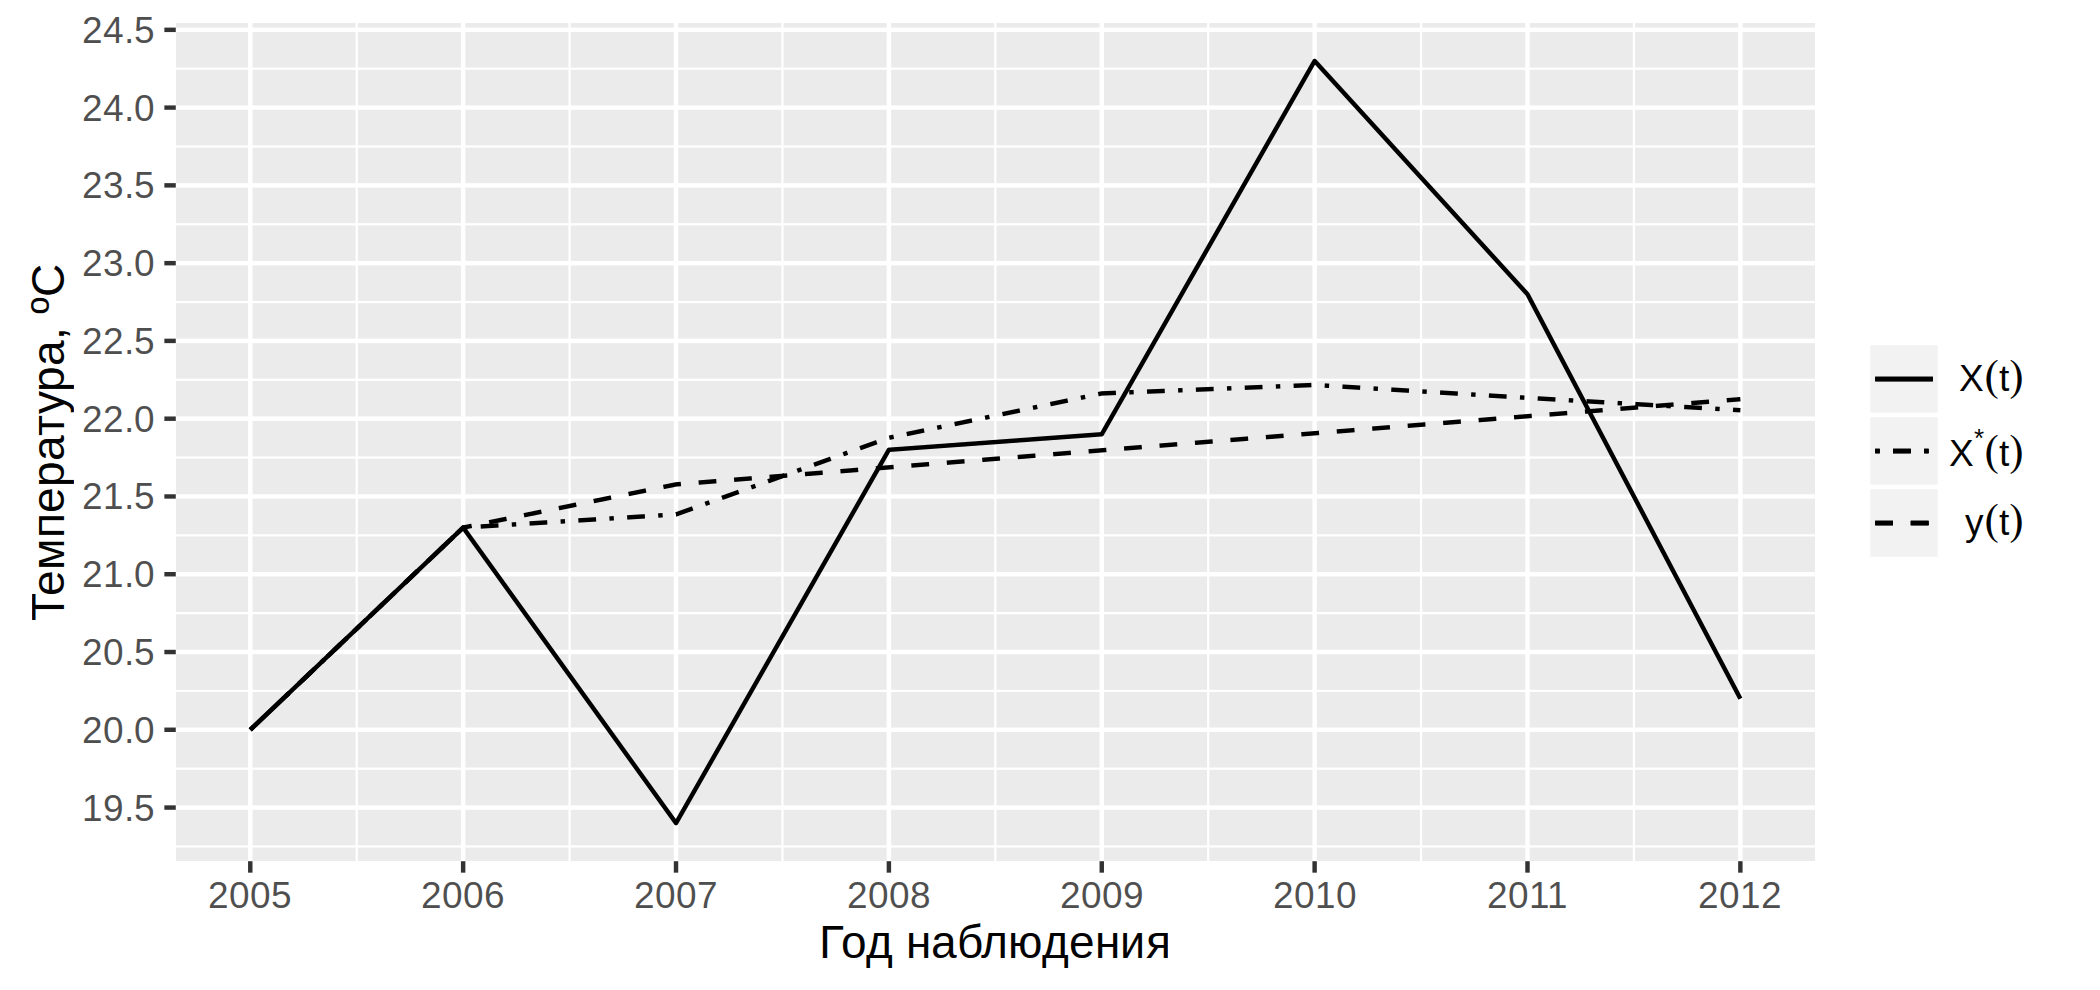
\includegraphics[width=0.95\textwidth]{../../figures/variogram/auto-rob-5-cross-prediction.png}
\end{frame}

\begin{frame}
  \frametitle{Заключение}

\end{frame}

\subsection{}
\begin{frame}
  \frametitle{}
  \begin{center}
    {\Huge Спасибо за внимание!}
  \end{center}
\end{frame}
\end{document}